
\chapter{Background}
%% { % STLCBOOL SCOPE

\newcommand{\stlcbool}{\ensuremath{\lambda_{\mathbb{B}}}\xspace}
\newcommand{\bool}{\text{bool}}
\newcommand{\true}{\textbf{true}\xspace}
\newcommand{\false}{\textbf{false}\xspace}
\newcommand{\ite}[3]{\textbf{if}~{#1}~\textbf{then}~{#2}~\textbf{else}~{#3}}
\newcommand{\typing}[3]{{#1} \vdash {#2} : {#3}}
\renewcommand{\eval}[2]{{#1} \longrightarrow {#2}}
\newcommand{\evals}[2]{{#1} \longrightarrow^* {#2}}

\chapter{Introduction}

The concept of programming can be defined as communicating how to perform tasks
to a computer. An increasing number of fields such as biology, engineering,
physics, psychology and sociology rely on programming. Programming is not
limited to sciences. The ubiquity of computers and the pervasive use of software
in our society indirectly depend on programming and programmers.  However,
software is notoriously unreliable. Given the extent of our dependence on
software this is all the more detrimental and costly.

In order to improve upon this situation we need to meliorate the process of
programming itself.
\begin{itemize}
\item 'Programming languages' are the tools/methods for programming
\item The minimum requirement is that a program does what it's intended to do.
\end{itemize}

For a programmer it is essential that she can validate that a program implements
exactly the intended task which is usually achieved by reasoning with the
\emph{expected behaviour} of a program.

But how is the behaviour of programming constructs defined, or more generally,
how are programming languages defined? The majority of programming languages
start with a reference implementation that effectively defines the language.
% Examples of languages that are (still) defined this way include Perl -
% Perl~5~\cite{perllanguage} and Python~\cite{pythonlanguage}.

After widespread use, a language may go through a standardization process:
multiple stakeholders develop a common language specification.
% , e.g. PHP was standardized in 2014~\cite{phpspec}.
Another approach is develop specifications together with a reference
implementation. These two approaches are not mutually exclusive: languages with
an existing specification are extended in tandem with implementations.

Such a language specification allows a programmer to resolve ambiguities when
reasoning about her programs independent of a particular implementation. It also
enables us to switch between implementations.

Programming language theory is a branch of computer science that deals with
language specifications, design, implementation, and in particular also
meta-theoretical analysis of programming languages, their semantics and related
systems like type-systems. When developing new languages or language features we
want to make sure that the design is coherent and fulfills the expectations of
users.

The programmer is often given useful safety guarantees for this programs. For
instance, many modern programming language provide garbage collection
facilities. Yet we want our programs to be memory safe, i.e. they do not access
memory that has been freed or that has not yet been initialized. Another safety
property is type-safety, i.e. the absence of dynamic type errors during
execution. These guarantees are usually provided for all programs written in a
language or a specific subset of programs, e.g. all type-checked programs. In a
meta-theoretical analysis we want to make sure that these are indeed valid
guarantees.

The meta-theory of programming language semantics and type-systems is highly
complex due to the management of many details and edge cases. As such, it is
prone to subtle errors that can invalidate large amounts of work.

For example, the Java programming language was long believed to be type-safe
\footnote{Except for some deliberate defects like the co-variance of arrays.}
but the addition of Generics made Java's type system in fact unsound
\cite{amin2016java}. Another problem concerns the type-checking of Java
programs. Generics made type-checking an undecidable property of
programs~\cite{grigore2017}. Decidability of type-checking does not have an
impact on properties that we get for type-checked programs, but for example it
opens up attack vectors on (web) services that deal with Java code because the
type-checker may run forever.

To increase the confidence in the correctness of formal meta-theory, techniques
for formalization in proof-assistants, also known as mechanization, have
received much attention. These systems allow us to state mathematical statements
and proofs for them and let the machine check that these are in fact valid
proofs. However, the high development cost of mechanizations continues to
prevent their widespread use. This leads us to the research question that this
thesis tries to answer:

\begin{center}
  \begin{minipage}{0.8\columnwidth}
    How can we reduce the costs of mechanizing formal meta-theory of programming
    languages?
  \end{minipage}
\end{center}

\begin{itemize}
\item Current methodology.
\item Why is the current methodology costly?
\item Give an idea of the relative effort.
\item What is the approach answer of this thesis?

  Increase reusability of code. Two strands: Modularity / Genericity.
\end{itemize}




The remainder of this chapter will give a more detailed introduction to the
relevant disciplines of specification, analysis and mechanization of programming
languages similar to what can be found in introductory textbooks such as
\cite{tapl}.

%% %-------------------------------------------------------------------------------
%% \section{Mechanization}
%% Mechanizing formal meta-theory in proof-assistants is crucial, both for the
%% increased confidence in complex designs and as a basis for technologies such as
%% proof-carrying code.  Formal reasoning in proof-assistants, also known as
%% mechanization, has high development costs.
%%

%% \begin{itemize}
%% \item
%%   Derive properties for all programs written in a language, like memory-safety,
%%   type-safety, resources-safety, termination, absence of deadlocks, race
%%   conditions and starvation.
%%
%% \item
%%   Prove correctness (preservation of semantics) of program analyses or compiler
%%   transformations.
%%
%%   by looking formally on the semantics, type systems and implementations like
%%   compilers or interpreters.
%% \end{itemize}

%-------------------------------------------------------------------------------
\section{Specifications}\label{sec:intro:specification}

%% Standardization and functional or program specifications are an essential
%% methodology in systems engineering and software development. It serves as the
%% baseline for correctness of implementations. Furthermore, multiple
%% implementations that are correct with respect to a common specification are
%% inter-operable or compatible to a certain extent. The precise meaning depends
%% on the context and the requirements.
%%
%% For programming languages for example, we want to guarantee that the same
%% program is executable by different implementations and performs the same
%% tasks.  This does for example also ensures that program analyses and program
%% transformations, e.g. for optimization, can be developed independent of a
%% particular implementation and adopted by multiple implementations.
%%
%% In this thesis, we are interested in programming languages themselves and not
%% so much interested in their implementations. Hence, a specification of a
%% application binary interface, for example, to achieve binary compatibility of
%% modules compiled by different compilers is beyond the scope of this thesis.

Specifications differ in the detail and precision they describe systems.
Industrial specifications of major programming languages are usually written in
natural language and are detailed to cover every aspect of the languages. The
use of natural language leaves opportunities for ambiguity, but disregarding
this problem, elaborate industrial specifications provide a good reference point
for language users and implementors. However, for meta-theoretical analyses more
rigorous specifications are necessary.

We will use \emph{formal specifications} and a mathematical language to
describe programming languages. This gives use the necessary precision and
avoids the ambiguities of natural languages. This section explains necessary
fundamental concepts for the formal specification of programming languages by
example of a small language \stlcbool: a simply-typed lambda calculus with
booleans. We specify the \emph{abstract syntax}, \emph{static type system} and
\emph{evaluation} of \stlcbool using inductive definitions. Along the way, we
define the terminology and notational conventions and make their meaning
precise.

%-------------------------------------------------------------------------------
\subsection{Syntax}\label{ssec:intro:syntax}

\begin{figure}[t]
  \centering
  \fbox{
    \begin{minipage}{\columnwidth}
    \begin{tabular}{lcll}
      $x,y$           & ::=    &                            & term variable    \\
      $\tau,\sigma$   & ::=    &                            & type             \\
                      & $\mid$ & $\tau \to \tau$            & function type    \\
                      & $\mid$ & $\bool$                    & boolean type     \\
      $e$             & ::=    &                            & term             \\
                      & $\mid$ & $\true$                    & true constant    \\
                      & $\mid$ & $\false$                   & false constant   \\
                      & $\mid$ & $\ite{e}{e}{e}$            & conditional      \\
                      & $\mid$ & $x$                        & term variable    \\
                      & $\mid$ & $\lambda x:\tau.e$         & term abstraction \\
                      & $\mid$ & $e~e$                      & application      \\
      $v$             & ::=    &                            & term             \\
                      & $\mid$ & $\true$                    & true constant    \\
                      & $\mid$ & $\false$                   & false constant   \\
                      & $\mid$ & $\lambda x:\tau.e$         & term abstraction \\
      $\Gamma$        & ::=    &                            & type context     \\
                      & $\mid$ & $\epsilon$                 & empty context    \\
                      & $\mid$ & $\Gamma, x:\tau$           & term binding     \\
    \end{tabular}
    \end{minipage}
  }
  \caption{\stlcbool syntax}
  \label{fig:intro:stlcboolsyntax}
\end{figure}

The syntax of \stlcbool is given in Figure \ref{fig:intro:stlcboolsyntax}. We
use a convention that is close to standard \textsc{EBnf} grammars. Elided in the
grammar are syntactic constructs like parentheses. We use parentheses freely to
resolve ambiguities in terms even if the grammar does not define them. Any
implementation that deals with the concrete syntax of a programming language has
of course to be more rigorous.

The grammar in Figure \ref{fig:intro:stlcboolsyntax} defines several
\emph{syntactic sorts} for \stlcbool. The \emph{meta-variable} $e$ stands for
expressions of \stlcbool of which there are 6 different kinds. An expression can
either be a boolean constant $\true$ or $\false$, a conditional form
$\ite{e_c}{e_t}{e_e}$, an \emph{object-language variable} (represented by the
meta-variable $x$), the definition of a function as a \textlambda-abstraction
$(\lambda x:\tau.e)$ or the application of an expression $e_1$ to another
expression $e_2$. Of course we only want to apply expressions $e_1$ that
represent functions: either by being a \textlambda-abstraction or evaluating to
one. Applying any \emph{value} other than a \textlambda-abstraction is a
\emph{type error}. We make this more precise below and come back to it it
Section \ref{sec:intro:typesafety} on analysis.

The grammar also includes the meta-variable $\tau$ that describes the types of
\stlcbool. Each \textlambda-abstraction contains a \emph{type annotation} $\tau$
for the argument variable $x$. The denotation is that the function represented
by the \textlambda-abstraction expects a value of type $\tau$ when it is
applied. We discuss types and typing contexts $\Gamma$ in more detail in Section
\ref{ssec:intro:typing} which deals with static typing.


%-------------------------------------------------------------------------------
\subsection{Semantics}\label{ssec:intro:semantics}

We have defined the syntax of \stlcbool expressions and can now turn towards
defining their meaning. There are multiple established ways to define semantics
of programming language. We can coarsely classify the approaches into three
different groups:

\begin{enumerate}
\item Operational Semantics

  Operational semantics defines the meaning of programs by specifying their
  execution in a state transition system. A \emph{state transition function} or
  a \emph{state transition relation} on the terms of the programming language
  defines the possible execution steps. The program is part of the state. For
  small languages the entire state might consist of only the program. After
  taking a step we are left with an updated state that includes a residual
  program.

  %% We can then define the meaning of programs to be the execution process on
  %% the abstract machine.


\item Denotational Semantics

  Denotational semantics defines the meaning of programs in terms of collection
  of \emph{mathematical semantic domains} that can include numbers, sets or
  functions. An \emph{interpretation function} maps program terms into these
  domains. This function is generally compositional in the syntax which
  is beneficial for modularity.

  Usually, the semantic domain has an established \emph{formal theory}. The
  theorems of the domain give rise to reasoning laws for programs. Furthermore,
  we can also derive properties of programming languages from properties of the
  collection of semantic domains.

\item Axiomatic Semantics

  Instead of deriving laws for programs from their execution behaviour or
  denotation we can also axiomatically assume these laws. This is known as an
  axiomatic semantics.

  This gives us immediately the means for reasoning about programs. Furthermore,
  we can derive a denotational semantics for the language by constructing a
  model that satisfies the chosen laws and derive properties for this model or
  even all models.

\end{enumerate}

These approaches have different trade-offs. Denotational and axiomatic semantics
immediately give us powerful mathematical tools to reason about programming
languages and their programs, but for larger languages the required technicality
and complexity makes it extremely difficult to even define a suitable semantics.

Operational semantics do not give us the same powerful mathematical reasoning
techniques and instead impose on us the laborious task to reason about programs
by observing their behaviour during execution. However, operational semantics
are simpler and easier to define than more abstract denotational or axiomatic
semantics. Moreover, they are much closer to actual implementations. Due to the
smaller gap, operational semantics make it easier to reason about the
correctness of implementations.

\begin{figure}[t]
  \centering
  \fbox{
    \begin{minipage}{\columnwidth}
      \framebox{\mbox{$\eval{e}{e}$}}\\
      \vspace{-5mm}
      \[ \begin{array}{c}
           \inferrule* [right=\textsc{EIfTrue},]
             {
             }
             {\eval{\ite{\true}{e_t}{e_e}}{e_t}
             } \\\\
           \inferrule* [right=\textsc{EIfFalse}]
             {
             }
             {\eval{\ite{\false}{e_t}{e_e}}{e_e}
             } \\\\
           \inferrule* [right=\textsc{EIf}]
             {\eval{e_c}{e_c'}
             }
             {\eval{\ite{e_c}{e_t}{e_e}}{\ite{e_c'}{e_t}{e_e}}
           } \\\\
           \inferrule* [right=\textsc{EAppAbs}]
             {
             }
             {\eval{(\lambda x:\tau.e_1)~e_2}{[x \mapsto e_2]e_1}
             } \\\\
           \inferrule* [right=\textsc{EApp}]
             {\eval{e_1}{e_2'}
             }
             {\eval{e_1~e_2}{e_1'~e_2}
             } \\\\
         \end{array}
       \]
    \end{minipage}
  }
  \caption{\stlcbool reduction rules}
  \label{fig:intro:stlcbooleval}
\end{figure}

For our \stlcbool language we define semantics using a \emph{small-step
  operational semantics}. This is also the approach used in Part \ref{part:gen}
of this thesis. Part \ref{part:mod} uses denotational semantics.

Figure \ref{fig:intro:stlcbooleval} gives the complete definition of the
operational semantics by means of an evaluation relation. The box in the upper
left corner \framebox{\mbox{$\eval{e_1}{e_2}$}} defines the shape and notation
that we use for the relation. In this case it is a binary relation between two
terms, which denotes that $e_1$ evaluates to $e_2$ in one step.

The remainder of the figure defines the relation using Gentzen-style inference
rules~\cite{gentzen1935}. In general, rules take the form
\[
  \inferrule* [right=\textsc{Name}]
    {J_1 \\ J_2 \\ \ldots \\ J_n
    }
    {J
    }
\]
where \textsc{Name} is an optional name for the rule that allows us to refer to
it. The meta-variable $J$ stands for judgements, which in our case are usually
mathematical statements in propositional or first-order logic. The judgements
$J_1, \ldots, J_n$ above the horizontal line are the premises of the rule, and
the judgement $J$ below the line is the conclusion. Rule without any premises
are also called \emph{axioms}. The conclusion will always involve the relation
that is being defined.

The single-step evaluation is defines using five rules. The two axioms
\textsc{EIfTrue} and \textsc{EIfFalse} show how to reduce an
\textbf{if}-expression in case the condition is either a \true or a \false
value. The case of a condition that is not yet fully evaluated is handled by
rule \textsc{EIf}. If the condition $e_c$ reduces to $e_c'$ in one step then we
can conclude the one step reduction
\[ \eval{\ite{e_c}{e_t}{e_e}}{\ite{e_c'}{e_t}{e_e}} \]

The last two rules cover the evaluation of \textlambda-terms. The rule
\textsc{EAppAbs} handles the case where the left-hand side of an application is
a \textlambda-term $(\lambda x:\tau.e_1)$. The residual program is the the body
$e_1$ of the function after substituting $e_2$ for $x$ which we write as
$[x \mapsto e_2]e_1$. The argument of the function does not have to be fully
evaluated, i.e. the rules encode a \emph{call-by-name} evaluation strategy. If
the left-hand side is not yet a \textlambda-term, we evaluate it first similarly
to \textsc{EIf}.

Note that this definition does not cover all the cases. In particular
the case of a \textlambda-term in the condition of an \textbf{if}-expression
\[ \ite{(\lambda x:\tau.e)}{e_t}{e_e} \]
\noindent and the cases of a boolean in the left-hand side of an application
\[ \true~e_1 \qquad \text{or} \qquad \false~e_2 \]
\noindent are not specified. Since no transition is defined and the execution
stopped without any \emph{meaningful result}, we also say that the evaluation
got stuck. In an implementation of the programming language, this corresponds to
an error that can happen during execution of a program. It's therefore also
called a \emph{(dynamic) type error}. Programmers want to detect potential
problems like that early in the development cycle and, if possible, at compile
time. This motivates the development of \emph{static type systems}.

%-------------------------------------------------------------------------------
\subsection{Typing}\label{ssec:intro:typing}

\begin{figure}[t]
  \centering
  \fbox{
    \begin{minipage}{\columnwidth}
      \framebox{\mbox{$\typing{\Gamma}{e}{\tau}$}}\\
      \vspace{-5mm}
      \[ \begin{array}{c}
           \inferrule* [right=\textsc{TTrue}]
             {
             }
             {\typing{\Gamma}{\true}{\bool}
             } \quad
           \inferrule* [right=\textsc{TFalse}]
             {
             }
             {\typing{\Gamma}{\false}{\bool}
             } \\\\
           \inferrule* [right=\textsc{TIf}]
             {\typing{\Gamma}{e_c}{\bool} \\
              \typing{\Gamma}{e_t}{\tau} \\
              \typing{\Gamma}{e_e}{\tau}
             }
             {\typing{\Gamma}{\ite{e_c}{e_t}{e_e}}{\tau}
             } \\\\
           \inferrule* [right=\textsc{TVar}]
             {x : \tau \in \Gamma
             }
             {\typing{\Gamma}{x}{\tau}
             } \quad
           \inferrule* [right=\textsc{TAbs}]
             {\typing{\Gamma,y:\sigma}{e}{\tau}
             }
             {\typing{\Gamma}{(\lambda y:\sigma. e)}{(\sigma\to\tau)}
             } \\\\
           \inferrule*[right=\textsc{TApp}]
             {\typing{\Gamma}{e_1}{\sigma \to \tau} \\
              \typing{\Gamma}{e_2}{\sigma}
             }
             {\typing{\Gamma}{e_1~e_2}{\tau}
             }
         \end{array}
       \]
    \end{minipage}
  }
  \caption{\stlcbool typing rules}
  \label{fig:intro:stlcbooltyping}
\end{figure}

A \emph{type system} is an assignment of types to expressions. Usually not all
expressions are typeable and un-typeable expressions are rejected. Also in some
languages there are expressions that can be assigned multiple, potentially
incomparable types. Both, the partiality and the ambiguity of types, suggests a
\emph{relational} rather than a \emph{functional} assignment. Such a relation is
defined in Figure \ref{fig:intro:stlcbooltyping}. It is a ternary relation
\framebox{\mbox{$\typing{\Gamma}{e}{\tau}$}} between a typing context $\Gamma$,
an expression $e$ and a type $\tau$.

The typing relation is defined using six rules. The two rules \textsc{TTrue} and
\textsc{TFalse} respectively state that the boolean constants $\true$ and
$\false$ have a boolean type. The rule \textsc{TIf} handles the case of an
\textbf{if}-expression. The three sub-expression position contain a
meta-variables $e_c$, $e_t$ and $e_e$. The premises require that the condition
$e_c$ has type boolean and the \textbf{then} and \textbf{else} branches have the
same type $\tau$. The rule then concludes that the entire \textbf{if}-expression
also has type $\tau$.

The three remaining rules deal with $\lambda$-abstractions. The typing context
$\Gamma$ is a list that associates term variables with types. In the case of a
variable, rule \textsc{TVar} looks up the corresponding type in $\Gamma$. Rule
\textsc{TAbs} checks the body of a $\lambda$-abstraction in the context
$(\Gamma,y:\sigma)$ which is the outside context $\Gamma$ extended with a pair
for the $lambda$-bound variable $y$. The type of the $\lambda$-abstraction is
the function type $(\sigma \to \tau)$ between the argument type $\sigma$ and the
type of the body $\tau$. Finally, rule \textsc{TApp} requires that the left
expressions of an application has a function type that is compatible with the
argument.

\paragraph{Example}
Consider the boolean negation function
\[
  \lambda y:\bool. \ite{y}{\false}{\true}
\]

This function sends booleans to booleans and should therefore have the type
$\bool\to\bool$. Giving the above typing relations, we can repeatedly apply the
rule to get a typing derivation for this. At each step only one possible rule
applies. We can arrange the rule applications in a so called \emph{derivation
  tree} that illustrates the whole derivation. Using the abbreviation
$\Gamma' := \Gamma, y:\bool$, we have the following tree:

\[
  \inferrule*
  { \inferrule*
    {
      \inferrule*{\;}{\typing{\Gamma'}{y}{\bool}} \\
      \inferrule*{\;}{\typing{\Gamma'}{\false}{\bool}} \\
      \inferrule*{\;}{\typing{\Gamma'}{\true}{\bool}} \\
    }
    {\typing{\Gamma'}{\ite{y}{\false}{\true}}{\bool}
    }
  }
  { \typing{\Gamma}{\lambda y:\bool. \ite{y}{\false}{\true}}{\bool \to \bool}
  }
\]


%-------------------------------------------------------------------------------
\section{Meta-Theoretical Analysis}\label{sec:intro:typesafety}

It is folklore in software development that bugs arise in both implementations
and in specifications. For instance, \cite{arts2015testing} describes a war
story on testing car software in which they found 227 bugs in the
\textsc{Autosar} specification (and in implementations).

To ensure that our languages are well-designed we want to establish
meta-theoretical properties that ensures that all the guarantees a user expects
are indeed valid. This needs a rigorous and formal analysis of the defined
semantics of a programming language. In this section we will look at the precise
definition of the type-safety language property, present methods for reasoning
about semantics and outline how these can be used to prove the type-safety
property for for our example calculus \stlcbool.

We previously characterized type-safety as the absence of type-errors during
execution. A type-error represents a state for which no further evaluation step
is defined and hence evaluation stopped.

\begin{defn}[Normal Form]
  An expression $e_1$ is a \emph{normal form} if no further execution step can be
  taken, i.e.
  \[ \forall e_2. \neg (\eval{e_1}{e_2}) \]
\end{defn}

A type-error however did not produce any \emph{meaningful result}. Let us define
what a meaningful result is. These are special expressions which are also called
values.

\begin{defn}[Value]
  Values are the subset of expressions that are defined by the following
  grammar:
  \begin{center}
    \begin{tabular}{lcll}
      $v$ & ::=    &                    & term             \\
          & $\mid$ & $\true$            & true constant    \\
          & $\mid$ & $\false$           & false constant   \\
          & $\mid$ & $\lambda x:\tau.e$ & term abstraction \\
    \end{tabular}
  \end{center}
\end{defn}

Expressions with type-errors are hence normal forms that are not values. We can
hence make \emph{the absence of type error} more precise by requiring that all
normal forms are already values.

\begin{thm}[Type-Safety]
  Let $\typing{\cdot}{e_1}{\tau}$. If $e_1$ evaluates to a normal form $e_2$
  then $e_2$ is a value.
\end{thm}

Note that this definition does not require the evaluation to terminate.  A
program that runs forever without a type-error is also considered type-safe.


\paragraph{Inductive Reasoning}
Figures \ref{fig:intro:stlcbooleval} and \ref{fig:intro:stlcbooltyping} define
evaluation and typing for \stlcbool. More precisely, our intention is to define
the \emph{smallest relation} that includes the presented rules. This gives rise
to a \emph{structural induction principle} for the relations. Put differently,
we can induct over the shape of derivation trees (or their size or height).

%% As an example consider the following determinacy theorem which states that
%% at each point there at most one possible successor state.
%% \begin{thm}[Determinacy]
%%   If $\eval{e_1}{e_2} \wedge \eval{e_1}{e_3}$ then $e_2 = e_3$.
%% \end{thm}


\begin{lem}[Progress]
  Let $\typing{\cdot}{e_1}{\tau}$. Either $e_1$ is a value or we can take another
  step, i.e.
  \[ \exists e_2. \eval{e_1}{e_2}. \]
\end{lem}


\begin{lem}[Preservation]
  If $\typing{\Gamma}{e_1}{\tau}$ and $\eval{e_1}{e_2}$ then $\typing{\Gamma}{e_2}{\tau}$.
\end{lem}




\section{Mechanization}

that he expects we need to

of languages on their own are not good enough to ensure a
good design.




The undecidability of type-checking Java~\cite{grigore2017} and the unsoundness
of its type system \cite{amin2016java} might be seen as bugs of the language
specification (but no formal specification of the complete Java language
exists).


A good approach is to develop software (and programming languages) in tandem
with an implementation and refine both. However, problems usually arise in
subtle edge cases that do not appear in normal program code that we write every
day and are easy to overlook in an





and such properties have only been established for subsets of the language such
as Featherweight Java \cite{igarashi2001featherweight}.

\begin{itemize}
\item
  Improving the correctness of C compilers is a worthy goal: C code is part of
  the trusted computing base for almost every modern computer system including
  mission-critical financial servers and life- critical pacemaker firmware.
\end{itemize}
From \cite{yang2011bugs}:

\blockquote{ The striking thing about our \textsc{CompCert} results is that the
  middle-end bugs we found in all other compilers are absent. As of early 2011,
  the under-development version of \textsc{CompCert} is the only compiler we
  have tested for which \textsc{Csmith} cannot find wrong-code errors. This is
  not for lack of trying: we have devoted about six CPU-years to the task. The
  apparent unbreakability of \textsc{CompCert} supports a strong argument that
  developing compiler optimizations within a proof framework, where safety
  checks are explicit and machine-checked, has tangible benefits for compiler
  users.}


%% The meta-theory of programming language semantics and type-systems is highly
%% complex due to the management of many details. Formal proofs are long and prone
%% to subtle errors that can invalidate large amounts of work. In order to
%% guarantee the correctness of formal meta-theory, techniques for mechanical
%% formalization in proof-assistants have received much attention in recent years.
%%
%% %-------------------------------------------------------------------------------
%% \section{Mechanization}
%% Mechanizing formal meta-theory in proof-assistants is crucial, both for the
%% increased confidence in complex designs and as a basis for technologies such as
%% proof-carrying code.  Formal reasoning in proof-assistants, also known as
%% mechanization, has high development costs.
%%
%% To lighten the burden of programming language mechanization, many
%% approaches have been developed that tackle the substantial boilerplate which
%% arises from variable binders. Unfortunately, the existing approaches are limited
%% in scope.
%% %% STEVEN: This is still valid, but I hope it's not misleading the reader into
%% %% thinking we deal with typing relations directly.
%% As a consequence, the human mechanizer is still unnecessarily burdened with
%% binder boilerplate and discouraged from taking on richer languages.
%%
%% This paper presents \Knot, a new approach that substantially extends the support
%% for binder boilerplate. \Knot is a highly expressive language for natural and
%% concise specification of syntax with binders. Its meta-theory constructively
%% guarantees the coverage of a considerable amount of binder boilerplate for
%% well-formed specifications, including that for well-scoping of terms and context
%% lookups. \Knot also comes with a code generator, \Needle, that specializes the
%% generic boilerplate for convenient embedding in \Coq and provides a tactic
%% library for automatically discharging proof obligations that frequently come up
%% in proofs of weakening and substitution lemmas of type-systems.
%%
%% Our evaluation shows, that Needle \& Knot significantly reduce the size of
%% language mechanizations (by 40\% in our case study). Moreover, as far as we
%% know, \Knot enables the most concise mechanization of the \POPLmark Challenge
%% (1a + 2a) and is two-thirds the size of the next smallest. Finally, \Knot allows
%% us to mechanize for instance dependently-typed languages, which is notoriously
%% challenging because of dependent contexts and mutually-recursive sorts with
%% variables.
%%
%% %-------------------------------------------------------------------------------
%% \section{Binding}
%%
%% To lighten the burden of programming language mechanization, many approaches
%% have been developed that tackle the substantial boilerplate which arises from
%% variable binders. Unfortunately, existing approaches for first-order
%% representations are limited to the boilerplate that concerns the syntax of
%% languages and do not tackle common boilerplate lemmas that arise for semantic
%% relations such as typing. Consequently, the human mechanizer is still burdened
%% with proving these substantial boilerplate lemmas manually.
%%
%% %% POPL 2014 Submission
%% %%
%% %%   A key concern in the mechanization of programming language metatheory is
%% %%   the representation of terms with variable binding. The properties of
%% %%   operations manipulating terms are notoriously burdensome to prove and the
%% %%   amount of work required to scale formalizations to realistic programming
%% %%   languages with rich binding forms is deemed infeasible. This is a pity,
%% %%   because we lose the practical benefits of mechanizing real programming
%% %%   languages.
%% %%
%% %%   We present a new solution to generically handle the boilerplate involved in
%% %%   mechanizations that scales to rich binding forms and advanced rules of
%% %%   scoping. We define a new specification language for abstract syntax with
%% %%   binding and implement a code generator that produces \Coq code for the
%% %%   representation of the abstract syntax, syntactic operations and proofs of
%% %%   their properties.
%% %%
%% %%   We illustrate how our approach removes the burden of variable binding
%% %%   boilerplate in the mechanization of realistic programming languages on a
%% %%   list of example specifications and a solution of the PoplMark challenge
%% %%   based on the generated code.

} % STLCBOOL SCOPE

\section{Overview}

\begin{center}
  \begin{minipage}{0.8\columnwidth}
    Keuchel, S., \& Schrijvers, T. (2013).
    \newblock Generic Datatypes à la Carte.
    \newblock In {\em Proceedings of the 9th ACM SIGPLAN workshop on Generic
      programming}, WGP ’13, pages 13-24. ACM.
  \end{minipage}
\end{center}

\begin{center}
  \begin{minipage}{0.8\columnwidth}
    Delaware, B., Keuchel, S., Schrijvers, T., and Oliveira,
    B. C. d.~S. (2013).
    \newblock Modular Monadic Meta-Theory.
    \newblock In {\em Proceedings of the 18th ACM SIGPLAN international
      conference on Functional programming}, ICFP '13, pages 319-330. ACM.
  \end{minipage}
\end{center}

\begin{center}
  \begin{minipage}{0.8\columnwidth}
    Keuchel, S. and Schrijvers, T. (2012).
    \newblock Modular Monadic Reasoning, a (Co-)Routine.
    \newblock Presented at \emph{the 24th Symposium on Implementation and
      Application of Functional Languages}, IFL '12.
  \end{minipage}
\end{center}


%%% Local Variables:
%%% mode: latex
%%% TeX-master: "../Main"
%%% End:

%% { % STLCBOOL SCOPE

\newcommand{\stlcbool}{\ensuremath{\lambda_{\mathbb{B}}}\xspace}
\newcommand{\bool}{\text{bool}}
\newcommand{\true}{\textbf{true}\xspace}
\newcommand{\false}{\textbf{false}\xspace}
\newcommand{\ite}[3]{\textbf{if}~{#1}~\textbf{then}~{#2}~\textbf{else}~{#3}}
\newcommand{\typing}[3]{{#1} \vdash {#2} : {#3}}
\renewcommand{\eval}[2]{{#1} \longrightarrow {#2}}
\newcommand{\evals}[2]{{#1} \longrightarrow^* {#2}}

\chapter{Introduction}

The concept of programming can be defined as communicating how to perform tasks
to a computer. An increasing number of fields such as biology, engineering,
physics, psychology and sociology rely on programming. Programming is not
limited to sciences. The ubiquity of computers and the pervasive use of software
in our society indirectly depend on programming and programmers.  However,
software is notoriously unreliable. Given the extent of our dependence on
software this is all the more detrimental and costly.

In order to improve upon this situation we need to meliorate the process of
programming itself.
\begin{itemize}
\item 'Programming languages' are the tools/methods for programming
\item The minimum requirement is that a program does what it's intended to do.
\end{itemize}

For a programmer it is essential that she can validate that a program implements
exactly the intended task which is usually achieved by reasoning with the
\emph{expected behaviour} of a program.

But how is the behaviour of programming constructs defined, or more generally,
how are programming languages defined? The majority of programming languages
start with a reference implementation that effectively defines the language.
% Examples of languages that are (still) defined this way include Perl -
% Perl~5~\cite{perllanguage} and Python~\cite{pythonlanguage}.

After widespread use, a language may go through a standardization process:
multiple stakeholders develop a common language specification.
% , e.g. PHP was standardized in 2014~\cite{phpspec}.
Another approach is develop specifications together with a reference
implementation. These two approaches are not mutually exclusive: languages with
an existing specification are extended in tandem with implementations.

Such a language specification allows a programmer to resolve ambiguities when
reasoning about her programs independent of a particular implementation. It also
enables us to switch between implementations.

Programming language theory is a branch of computer science that deals with
language specifications, design, implementation, and in particular also
meta-theoretical analysis of programming languages, their semantics and related
systems like type-systems. When developing new languages or language features we
want to make sure that the design is coherent and fulfills the expectations of
users.

The programmer is often given useful safety guarantees for this programs. For
instance, many modern programming language provide garbage collection
facilities. Yet we want our programs to be memory safe, i.e. they do not access
memory that has been freed or that has not yet been initialized. Another safety
property is type-safety, i.e. the absence of dynamic type errors during
execution. These guarantees are usually provided for all programs written in a
language or a specific subset of programs, e.g. all type-checked programs. In a
meta-theoretical analysis we want to make sure that these are indeed valid
guarantees.

The meta-theory of programming language semantics and type-systems is highly
complex due to the management of many details and edge cases. As such, it is
prone to subtle errors that can invalidate large amounts of work.

For example, the Java programming language was long believed to be type-safe
\footnote{Except for some deliberate defects like the co-variance of arrays.}
but the addition of Generics made Java's type system in fact unsound
\cite{amin2016java}. Another problem concerns the type-checking of Java
programs. Generics made type-checking an undecidable property of
programs~\cite{grigore2017}. Decidability of type-checking does not have an
impact on properties that we get for type-checked programs, but for example it
opens up attack vectors on (web) services that deal with Java code because the
type-checker may run forever.

To increase the confidence in the correctness of formal meta-theory, techniques
for formalization in proof-assistants, also known as mechanization, have
received much attention. These systems allow us to state mathematical statements
and proofs for them and let the machine check that these are in fact valid
proofs. However, the high development cost of mechanizations continues to
prevent their widespread use. This leads us to the research question that this
thesis tries to answer:

\begin{center}
  \begin{minipage}{0.8\columnwidth}
    How can we reduce the costs of mechanizing formal meta-theory of programming
    languages?
  \end{minipage}
\end{center}

\begin{itemize}
\item Current methodology.
\item Why is the current methodology costly?
\item Give an idea of the relative effort.
\item What is the approach answer of this thesis?

  Increase reusability of code. Two strands: Modularity / Genericity.
\end{itemize}




The remainder of this chapter will give a more detailed introduction to the
relevant disciplines of specification, analysis and mechanization of programming
languages similar to what can be found in introductory textbooks such as
\cite{tapl}.

%% %-------------------------------------------------------------------------------
%% \section{Mechanization}
%% Mechanizing formal meta-theory in proof-assistants is crucial, both for the
%% increased confidence in complex designs and as a basis for technologies such as
%% proof-carrying code.  Formal reasoning in proof-assistants, also known as
%% mechanization, has high development costs.
%%

%% \begin{itemize}
%% \item
%%   Derive properties for all programs written in a language, like memory-safety,
%%   type-safety, resources-safety, termination, absence of deadlocks, race
%%   conditions and starvation.
%%
%% \item
%%   Prove correctness (preservation of semantics) of program analyses or compiler
%%   transformations.
%%
%%   by looking formally on the semantics, type systems and implementations like
%%   compilers or interpreters.
%% \end{itemize}

%-------------------------------------------------------------------------------
\section{Specifications}\label{sec:intro:specification}

%% Standardization and functional or program specifications are an essential
%% methodology in systems engineering and software development. It serves as the
%% baseline for correctness of implementations. Furthermore, multiple
%% implementations that are correct with respect to a common specification are
%% inter-operable or compatible to a certain extent. The precise meaning depends
%% on the context and the requirements.
%%
%% For programming languages for example, we want to guarantee that the same
%% program is executable by different implementations and performs the same
%% tasks.  This does for example also ensures that program analyses and program
%% transformations, e.g. for optimization, can be developed independent of a
%% particular implementation and adopted by multiple implementations.
%%
%% In this thesis, we are interested in programming languages themselves and not
%% so much interested in their implementations. Hence, a specification of a
%% application binary interface, for example, to achieve binary compatibility of
%% modules compiled by different compilers is beyond the scope of this thesis.

Specifications differ in the detail and precision they describe systems.
Industrial specifications of major programming languages are usually written in
natural language and are detailed to cover every aspect of the languages. The
use of natural language leaves opportunities for ambiguity, but disregarding
this problem, elaborate industrial specifications provide a good reference point
for language users and implementors. However, for meta-theoretical analyses more
rigorous specifications are necessary.

We will use \emph{formal specifications} and a mathematical language to
describe programming languages. This gives use the necessary precision and
avoids the ambiguities of natural languages. This section explains necessary
fundamental concepts for the formal specification of programming languages by
example of a small language \stlcbool: a simply-typed lambda calculus with
booleans. We specify the \emph{abstract syntax}, \emph{static type system} and
\emph{evaluation} of \stlcbool using inductive definitions. Along the way, we
define the terminology and notational conventions and make their meaning
precise.

%-------------------------------------------------------------------------------
\subsection{Syntax}\label{ssec:intro:syntax}

\begin{figure}[t]
  \centering
  \fbox{
    \begin{minipage}{\columnwidth}
    \begin{tabular}{lcll}
      $x,y$           & ::=    &                            & term variable    \\
      $\tau,\sigma$   & ::=    &                            & type             \\
                      & $\mid$ & $\tau \to \tau$            & function type    \\
                      & $\mid$ & $\bool$                    & boolean type     \\
      $e$             & ::=    &                            & term             \\
                      & $\mid$ & $\true$                    & true constant    \\
                      & $\mid$ & $\false$                   & false constant   \\
                      & $\mid$ & $\ite{e}{e}{e}$            & conditional      \\
                      & $\mid$ & $x$                        & term variable    \\
                      & $\mid$ & $\lambda x:\tau.e$         & term abstraction \\
                      & $\mid$ & $e~e$                      & application      \\
      $v$             & ::=    &                            & term             \\
                      & $\mid$ & $\true$                    & true constant    \\
                      & $\mid$ & $\false$                   & false constant   \\
                      & $\mid$ & $\lambda x:\tau.e$         & term abstraction \\
      $\Gamma$        & ::=    &                            & type context     \\
                      & $\mid$ & $\epsilon$                 & empty context    \\
                      & $\mid$ & $\Gamma, x:\tau$           & term binding     \\
    \end{tabular}
    \end{minipage}
  }
  \caption{\stlcbool syntax}
  \label{fig:intro:stlcboolsyntax}
\end{figure}

The syntax of \stlcbool is given in Figure \ref{fig:intro:stlcboolsyntax}. We
use a convention that is close to standard \textsc{EBnf} grammars. Elided in the
grammar are syntactic constructs like parentheses. We use parentheses freely to
resolve ambiguities in terms even if the grammar does not define them. Any
implementation that deals with the concrete syntax of a programming language has
of course to be more rigorous.

The grammar in Figure \ref{fig:intro:stlcboolsyntax} defines several
\emph{syntactic sorts} for \stlcbool. The \emph{meta-variable} $e$ stands for
expressions of \stlcbool of which there are 6 different kinds. An expression can
either be a boolean constant $\true$ or $\false$, a conditional form
$\ite{e_c}{e_t}{e_e}$, an \emph{object-language variable} (represented by the
meta-variable $x$), the definition of a function as a \textlambda-abstraction
$(\lambda x:\tau.e)$ or the application of an expression $e_1$ to another
expression $e_2$. Of course we only want to apply expressions $e_1$ that
represent functions: either by being a \textlambda-abstraction or evaluating to
one. Applying any \emph{value} other than a \textlambda-abstraction is a
\emph{type error}. We make this more precise below and come back to it it
Section \ref{sec:intro:typesafety} on analysis.

The grammar also includes the meta-variable $\tau$ that describes the types of
\stlcbool. Each \textlambda-abstraction contains a \emph{type annotation} $\tau$
for the argument variable $x$. The denotation is that the function represented
by the \textlambda-abstraction expects a value of type $\tau$ when it is
applied. We discuss types and typing contexts $\Gamma$ in more detail in Section
\ref{ssec:intro:typing} which deals with static typing.


%-------------------------------------------------------------------------------
\subsection{Semantics}\label{ssec:intro:semantics}

We have defined the syntax of \stlcbool expressions and can now turn towards
defining their meaning. There are multiple established ways to define semantics
of programming language. We can coarsely classify the approaches into three
different groups:

\begin{enumerate}
\item Operational Semantics

  Operational semantics defines the meaning of programs by specifying their
  execution in a state transition system. A \emph{state transition function} or
  a \emph{state transition relation} on the terms of the programming language
  defines the possible execution steps. The program is part of the state. For
  small languages the entire state might consist of only the program. After
  taking a step we are left with an updated state that includes a residual
  program.

  %% We can then define the meaning of programs to be the execution process on
  %% the abstract machine.


\item Denotational Semantics

  Denotational semantics defines the meaning of programs in terms of collection
  of \emph{mathematical semantic domains} that can include numbers, sets or
  functions. An \emph{interpretation function} maps program terms into these
  domains. This function is generally compositional in the syntax which
  is beneficial for modularity.

  Usually, the semantic domain has an established \emph{formal theory}. The
  theorems of the domain give rise to reasoning laws for programs. Furthermore,
  we can also derive properties of programming languages from properties of the
  collection of semantic domains.

\item Axiomatic Semantics

  Instead of deriving laws for programs from their execution behaviour or
  denotation we can also axiomatically assume these laws. This is known as an
  axiomatic semantics.

  This gives us immediately the means for reasoning about programs. Furthermore,
  we can derive a denotational semantics for the language by constructing a
  model that satisfies the chosen laws and derive properties for this model or
  even all models.

\end{enumerate}

These approaches have different trade-offs. Denotational and axiomatic semantics
immediately give us powerful mathematical tools to reason about programming
languages and their programs, but for larger languages the required technicality
and complexity makes it extremely difficult to even define a suitable semantics.

Operational semantics do not give us the same powerful mathematical reasoning
techniques and instead impose on us the laborious task to reason about programs
by observing their behaviour during execution. However, operational semantics
are simpler and easier to define than more abstract denotational or axiomatic
semantics. Moreover, they are much closer to actual implementations. Due to the
smaller gap, operational semantics make it easier to reason about the
correctness of implementations.

\begin{figure}[t]
  \centering
  \fbox{
    \begin{minipage}{\columnwidth}
      \framebox{\mbox{$\eval{e}{e}$}}\\
      \vspace{-5mm}
      \[ \begin{array}{c}
           \inferrule* [right=\textsc{EIfTrue},]
             {
             }
             {\eval{\ite{\true}{e_t}{e_e}}{e_t}
             } \\\\
           \inferrule* [right=\textsc{EIfFalse}]
             {
             }
             {\eval{\ite{\false}{e_t}{e_e}}{e_e}
             } \\\\
           \inferrule* [right=\textsc{EIf}]
             {\eval{e_c}{e_c'}
             }
             {\eval{\ite{e_c}{e_t}{e_e}}{\ite{e_c'}{e_t}{e_e}}
           } \\\\
           \inferrule* [right=\textsc{EAppAbs}]
             {
             }
             {\eval{(\lambda x:\tau.e_1)~e_2}{[x \mapsto e_2]e_1}
             } \\\\
           \inferrule* [right=\textsc{EApp}]
             {\eval{e_1}{e_2'}
             }
             {\eval{e_1~e_2}{e_1'~e_2}
             } \\\\
         \end{array}
       \]
    \end{minipage}
  }
  \caption{\stlcbool reduction rules}
  \label{fig:intro:stlcbooleval}
\end{figure}

For our \stlcbool language we define semantics using a \emph{small-step
  operational semantics}. This is also the approach used in Part \ref{part:gen}
of this thesis. Part \ref{part:mod} uses denotational semantics.

Figure \ref{fig:intro:stlcbooleval} gives the complete definition of the
operational semantics by means of an evaluation relation. The box in the upper
left corner \framebox{\mbox{$\eval{e_1}{e_2}$}} defines the shape and notation
that we use for the relation. In this case it is a binary relation between two
terms, which denotes that $e_1$ evaluates to $e_2$ in one step.

The remainder of the figure defines the relation using Gentzen-style inference
rules~\cite{gentzen1935}. In general, rules take the form
\[
  \inferrule* [right=\textsc{Name}]
    {J_1 \\ J_2 \\ \ldots \\ J_n
    }
    {J
    }
\]
where \textsc{Name} is an optional name for the rule that allows us to refer to
it. The meta-variable $J$ stands for judgements, which in our case are usually
mathematical statements in propositional or first-order logic. The judgements
$J_1, \ldots, J_n$ above the horizontal line are the premises of the rule, and
the judgement $J$ below the line is the conclusion. Rule without any premises
are also called \emph{axioms}. The conclusion will always involve the relation
that is being defined.

The single-step evaluation is defines using five rules. The two axioms
\textsc{EIfTrue} and \textsc{EIfFalse} show how to reduce an
\textbf{if}-expression in case the condition is either a \true or a \false
value. The case of a condition that is not yet fully evaluated is handled by
rule \textsc{EIf}. If the condition $e_c$ reduces to $e_c'$ in one step then we
can conclude the one step reduction
\[ \eval{\ite{e_c}{e_t}{e_e}}{\ite{e_c'}{e_t}{e_e}} \]

The last two rules cover the evaluation of \textlambda-terms. The rule
\textsc{EAppAbs} handles the case where the left-hand side of an application is
a \textlambda-term $(\lambda x:\tau.e_1)$. The residual program is the the body
$e_1$ of the function after substituting $e_2$ for $x$ which we write as
$[x \mapsto e_2]e_1$. The argument of the function does not have to be fully
evaluated, i.e. the rules encode a \emph{call-by-name} evaluation strategy. If
the left-hand side is not yet a \textlambda-term, we evaluate it first similarly
to \textsc{EIf}.

Note that this definition does not cover all the cases. In particular
the case of a \textlambda-term in the condition of an \textbf{if}-expression
\[ \ite{(\lambda x:\tau.e)}{e_t}{e_e} \]
\noindent and the cases of a boolean in the left-hand side of an application
\[ \true~e_1 \qquad \text{or} \qquad \false~e_2 \]
\noindent are not specified. Since no transition is defined and the execution
stopped without any \emph{meaningful result}, we also say that the evaluation
got stuck. In an implementation of the programming language, this corresponds to
an error that can happen during execution of a program. It's therefore also
called a \emph{(dynamic) type error}. Programmers want to detect potential
problems like that early in the development cycle and, if possible, at compile
time. This motivates the development of \emph{static type systems}.

%-------------------------------------------------------------------------------
\subsection{Typing}\label{ssec:intro:typing}

\begin{figure}[t]
  \centering
  \fbox{
    \begin{minipage}{\columnwidth}
      \framebox{\mbox{$\typing{\Gamma}{e}{\tau}$}}\\
      \vspace{-5mm}
      \[ \begin{array}{c}
           \inferrule* [right=\textsc{TTrue}]
             {
             }
             {\typing{\Gamma}{\true}{\bool}
             } \quad
           \inferrule* [right=\textsc{TFalse}]
             {
             }
             {\typing{\Gamma}{\false}{\bool}
             } \\\\
           \inferrule* [right=\textsc{TIf}]
             {\typing{\Gamma}{e_c}{\bool} \\
              \typing{\Gamma}{e_t}{\tau} \\
              \typing{\Gamma}{e_e}{\tau}
             }
             {\typing{\Gamma}{\ite{e_c}{e_t}{e_e}}{\tau}
             } \\\\
           \inferrule* [right=\textsc{TVar}]
             {x : \tau \in \Gamma
             }
             {\typing{\Gamma}{x}{\tau}
             } \quad
           \inferrule* [right=\textsc{TAbs}]
             {\typing{\Gamma,y:\sigma}{e}{\tau}
             }
             {\typing{\Gamma}{(\lambda y:\sigma. e)}{(\sigma\to\tau)}
             } \\\\
           \inferrule*[right=\textsc{TApp}]
             {\typing{\Gamma}{e_1}{\sigma \to \tau} \\
              \typing{\Gamma}{e_2}{\sigma}
             }
             {\typing{\Gamma}{e_1~e_2}{\tau}
             }
         \end{array}
       \]
    \end{minipage}
  }
  \caption{\stlcbool typing rules}
  \label{fig:intro:stlcbooltyping}
\end{figure}

A \emph{type system} is an assignment of types to expressions. Usually not all
expressions are typeable and un-typeable expressions are rejected. Also in some
languages there are expressions that can be assigned multiple, potentially
incomparable types. Both, the partiality and the ambiguity of types, suggests a
\emph{relational} rather than a \emph{functional} assignment. Such a relation is
defined in Figure \ref{fig:intro:stlcbooltyping}. It is a ternary relation
\framebox{\mbox{$\typing{\Gamma}{e}{\tau}$}} between a typing context $\Gamma$,
an expression $e$ and a type $\tau$.

The typing relation is defined using six rules. The two rules \textsc{TTrue} and
\textsc{TFalse} respectively state that the boolean constants $\true$ and
$\false$ have a boolean type. The rule \textsc{TIf} handles the case of an
\textbf{if}-expression. The three sub-expression position contain a
meta-variables $e_c$, $e_t$ and $e_e$. The premises require that the condition
$e_c$ has type boolean and the \textbf{then} and \textbf{else} branches have the
same type $\tau$. The rule then concludes that the entire \textbf{if}-expression
also has type $\tau$.

The three remaining rules deal with $\lambda$-abstractions. The typing context
$\Gamma$ is a list that associates term variables with types. In the case of a
variable, rule \textsc{TVar} looks up the corresponding type in $\Gamma$. Rule
\textsc{TAbs} checks the body of a $\lambda$-abstraction in the context
$(\Gamma,y:\sigma)$ which is the outside context $\Gamma$ extended with a pair
for the $lambda$-bound variable $y$. The type of the $\lambda$-abstraction is
the function type $(\sigma \to \tau)$ between the argument type $\sigma$ and the
type of the body $\tau$. Finally, rule \textsc{TApp} requires that the left
expressions of an application has a function type that is compatible with the
argument.

\paragraph{Example}
Consider the boolean negation function
\[
  \lambda y:\bool. \ite{y}{\false}{\true}
\]

This function sends booleans to booleans and should therefore have the type
$\bool\to\bool$. Giving the above typing relations, we can repeatedly apply the
rule to get a typing derivation for this. At each step only one possible rule
applies. We can arrange the rule applications in a so called \emph{derivation
  tree} that illustrates the whole derivation. Using the abbreviation
$\Gamma' := \Gamma, y:\bool$, we have the following tree:

\[
  \inferrule*
  { \inferrule*
    {
      \inferrule*{\;}{\typing{\Gamma'}{y}{\bool}} \\
      \inferrule*{\;}{\typing{\Gamma'}{\false}{\bool}} \\
      \inferrule*{\;}{\typing{\Gamma'}{\true}{\bool}} \\
    }
    {\typing{\Gamma'}{\ite{y}{\false}{\true}}{\bool}
    }
  }
  { \typing{\Gamma}{\lambda y:\bool. \ite{y}{\false}{\true}}{\bool \to \bool}
  }
\]


%-------------------------------------------------------------------------------
\section{Meta-Theoretical Analysis}\label{sec:intro:typesafety}

It is folklore in software development that bugs arise in both implementations
and in specifications. For instance, \cite{arts2015testing} describes a war
story on testing car software in which they found 227 bugs in the
\textsc{Autosar} specification (and in implementations).

To ensure that our languages are well-designed we want to establish
meta-theoretical properties that ensures that all the guarantees a user expects
are indeed valid. This needs a rigorous and formal analysis of the defined
semantics of a programming language. In this section we will look at the precise
definition of the type-safety language property, present methods for reasoning
about semantics and outline how these can be used to prove the type-safety
property for for our example calculus \stlcbool.

We previously characterized type-safety as the absence of type-errors during
execution. A type-error represents a state for which no further evaluation step
is defined and hence evaluation stopped.

\begin{defn}[Normal Form]
  An expression $e_1$ is a \emph{normal form} if no further execution step can be
  taken, i.e.
  \[ \forall e_2. \neg (\eval{e_1}{e_2}) \]
\end{defn}

A type-error however did not produce any \emph{meaningful result}. Let us define
what a meaningful result is. These are special expressions which are also called
values.

\begin{defn}[Value]
  Values are the subset of expressions that are defined by the following
  grammar:
  \begin{center}
    \begin{tabular}{lcll}
      $v$ & ::=    &                    & term             \\
          & $\mid$ & $\true$            & true constant    \\
          & $\mid$ & $\false$           & false constant   \\
          & $\mid$ & $\lambda x:\tau.e$ & term abstraction \\
    \end{tabular}
  \end{center}
\end{defn}

Expressions with type-errors are hence normal forms that are not values. We can
hence make \emph{the absence of type error} more precise by requiring that all
normal forms are already values.

\begin{thm}[Type-Safety]
  Let $\typing{\cdot}{e_1}{\tau}$. If $e_1$ evaluates to a normal form $e_2$
  then $e_2$ is a value.
\end{thm}

Note that this definition does not require the evaluation to terminate.  A
program that runs forever without a type-error is also considered type-safe.


\paragraph{Inductive Reasoning}
Figures \ref{fig:intro:stlcbooleval} and \ref{fig:intro:stlcbooltyping} define
evaluation and typing for \stlcbool. More precisely, our intention is to define
the \emph{smallest relation} that includes the presented rules. This gives rise
to a \emph{structural induction principle} for the relations. Put differently,
we can induct over the shape of derivation trees (or their size or height).

%% As an example consider the following determinacy theorem which states that
%% at each point there at most one possible successor state.
%% \begin{thm}[Determinacy]
%%   If $\eval{e_1}{e_2} \wedge \eval{e_1}{e_3}$ then $e_2 = e_3$.
%% \end{thm}


\begin{lem}[Progress]
  Let $\typing{\cdot}{e_1}{\tau}$. Either $e_1$ is a value or we can take another
  step, i.e.
  \[ \exists e_2. \eval{e_1}{e_2}. \]
\end{lem}


\begin{lem}[Preservation]
  If $\typing{\Gamma}{e_1}{\tau}$ and $\eval{e_1}{e_2}$ then $\typing{\Gamma}{e_2}{\tau}$.
\end{lem}




\section{Mechanization}

that he expects we need to

of languages on their own are not good enough to ensure a
good design.




The undecidability of type-checking Java~\cite{grigore2017} and the unsoundness
of its type system \cite{amin2016java} might be seen as bugs of the language
specification (but no formal specification of the complete Java language
exists).


A good approach is to develop software (and programming languages) in tandem
with an implementation and refine both. However, problems usually arise in
subtle edge cases that do not appear in normal program code that we write every
day and are easy to overlook in an





and such properties have only been established for subsets of the language such
as Featherweight Java \cite{igarashi2001featherweight}.

\begin{itemize}
\item
  Improving the correctness of C compilers is a worthy goal: C code is part of
  the trusted computing base for almost every modern computer system including
  mission-critical financial servers and life- critical pacemaker firmware.
\end{itemize}
From \cite{yang2011bugs}:

\blockquote{ The striking thing about our \textsc{CompCert} results is that the
  middle-end bugs we found in all other compilers are absent. As of early 2011,
  the under-development version of \textsc{CompCert} is the only compiler we
  have tested for which \textsc{Csmith} cannot find wrong-code errors. This is
  not for lack of trying: we have devoted about six CPU-years to the task. The
  apparent unbreakability of \textsc{CompCert} supports a strong argument that
  developing compiler optimizations within a proof framework, where safety
  checks are explicit and machine-checked, has tangible benefits for compiler
  users.}


%% The meta-theory of programming language semantics and type-systems is highly
%% complex due to the management of many details. Formal proofs are long and prone
%% to subtle errors that can invalidate large amounts of work. In order to
%% guarantee the correctness of formal meta-theory, techniques for mechanical
%% formalization in proof-assistants have received much attention in recent years.
%%
%% %-------------------------------------------------------------------------------
%% \section{Mechanization}
%% Mechanizing formal meta-theory in proof-assistants is crucial, both for the
%% increased confidence in complex designs and as a basis for technologies such as
%% proof-carrying code.  Formal reasoning in proof-assistants, also known as
%% mechanization, has high development costs.
%%
%% To lighten the burden of programming language mechanization, many
%% approaches have been developed that tackle the substantial boilerplate which
%% arises from variable binders. Unfortunately, the existing approaches are limited
%% in scope.
%% %% STEVEN: This is still valid, but I hope it's not misleading the reader into
%% %% thinking we deal with typing relations directly.
%% As a consequence, the human mechanizer is still unnecessarily burdened with
%% binder boilerplate and discouraged from taking on richer languages.
%%
%% This paper presents \Knot, a new approach that substantially extends the support
%% for binder boilerplate. \Knot is a highly expressive language for natural and
%% concise specification of syntax with binders. Its meta-theory constructively
%% guarantees the coverage of a considerable amount of binder boilerplate for
%% well-formed specifications, including that for well-scoping of terms and context
%% lookups. \Knot also comes with a code generator, \Needle, that specializes the
%% generic boilerplate for convenient embedding in \Coq and provides a tactic
%% library for automatically discharging proof obligations that frequently come up
%% in proofs of weakening and substitution lemmas of type-systems.
%%
%% Our evaluation shows, that Needle \& Knot significantly reduce the size of
%% language mechanizations (by 40\% in our case study). Moreover, as far as we
%% know, \Knot enables the most concise mechanization of the \POPLmark Challenge
%% (1a + 2a) and is two-thirds the size of the next smallest. Finally, \Knot allows
%% us to mechanize for instance dependently-typed languages, which is notoriously
%% challenging because of dependent contexts and mutually-recursive sorts with
%% variables.
%%
%% %-------------------------------------------------------------------------------
%% \section{Binding}
%%
%% To lighten the burden of programming language mechanization, many approaches
%% have been developed that tackle the substantial boilerplate which arises from
%% variable binders. Unfortunately, existing approaches for first-order
%% representations are limited to the boilerplate that concerns the syntax of
%% languages and do not tackle common boilerplate lemmas that arise for semantic
%% relations such as typing. Consequently, the human mechanizer is still burdened
%% with proving these substantial boilerplate lemmas manually.
%%
%% %% POPL 2014 Submission
%% %%
%% %%   A key concern in the mechanization of programming language metatheory is
%% %%   the representation of terms with variable binding. The properties of
%% %%   operations manipulating terms are notoriously burdensome to prove and the
%% %%   amount of work required to scale formalizations to realistic programming
%% %%   languages with rich binding forms is deemed infeasible. This is a pity,
%% %%   because we lose the practical benefits of mechanizing real programming
%% %%   languages.
%% %%
%% %%   We present a new solution to generically handle the boilerplate involved in
%% %%   mechanizations that scales to rich binding forms and advanced rules of
%% %%   scoping. We define a new specification language for abstract syntax with
%% %%   binding and implement a code generator that produces \Coq code for the
%% %%   representation of the abstract syntax, syntactic operations and proofs of
%% %%   their properties.
%% %%
%% %%   We illustrate how our approach removes the burden of variable binding
%% %%   boilerplate in the mechanization of realistic programming languages on a
%% %%   list of example specifications and a solution of the PoplMark challenge
%% %%   based on the generated code.

} % STLCBOOL SCOPE

\section{Overview}

\begin{center}
  \begin{minipage}{0.8\columnwidth}
    Keuchel, S., \& Schrijvers, T. (2013).
    \newblock Generic Datatypes à la Carte.
    \newblock In {\em Proceedings of the 9th ACM SIGPLAN workshop on Generic
      programming}, WGP ’13, pages 13-24. ACM.
  \end{minipage}
\end{center}

\begin{center}
  \begin{minipage}{0.8\columnwidth}
    Delaware, B., Keuchel, S., Schrijvers, T., and Oliveira,
    B. C. d.~S. (2013).
    \newblock Modular Monadic Meta-Theory.
    \newblock In {\em Proceedings of the 18th ACM SIGPLAN international
      conference on Functional programming}, ICFP '13, pages 319-330. ACM.
  \end{minipage}
\end{center}

\begin{center}
  \begin{minipage}{0.8\columnwidth}
    Keuchel, S. and Schrijvers, T. (2012).
    \newblock Modular Monadic Reasoning, a (Co-)Routine.
    \newblock Presented at \emph{the 24th Symposium on Implementation and
      Application of Functional Languages}, IFL '12.
  \end{minipage}
\end{center}


%%% Local Variables:
%%% mode: latex
%%% TeX-master: "../Main"
%%% End:

%% \clearpage
%% ODER: format ==         = "\mathrel{==}"
%% ODER: format /=         = "\neq "
%
%
\makeatletter
\@ifundefined{lhs2tex.lhs2tex.sty.read}%
  {\@namedef{lhs2tex.lhs2tex.sty.read}{}%
   \newcommand\SkipToFmtEnd{}%
   \newcommand\EndFmtInput{}%
   \long\def\SkipToFmtEnd#1\EndFmtInput{}%
  }\SkipToFmtEnd

\newcommand\ReadOnlyOnce[1]{\@ifundefined{#1}{\@namedef{#1}{}}\SkipToFmtEnd}
\usepackage{amstext}
\usepackage{amssymb}
\usepackage{stmaryrd}
\DeclareFontFamily{OT1}{cmtex}{}
\DeclareFontShape{OT1}{cmtex}{m}{n}
  {<5><6><7><8>cmtex8
   <9>cmtex9
   <10><10.95><12><14.4><17.28><20.74><24.88>cmtex10}{}
\DeclareFontShape{OT1}{cmtex}{m}{it}
  {<-> ssub * cmtt/m/it}{}
\newcommand{\texfamily}{\fontfamily{cmtex}\selectfont}
\DeclareFontShape{OT1}{cmtt}{bx}{n}
  {<5><6><7><8>cmtt8
   <9>cmbtt9
   <10><10.95><12><14.4><17.28><20.74><24.88>cmbtt10}{}
\DeclareFontShape{OT1}{cmtex}{bx}{n}
  {<-> ssub * cmtt/bx/n}{}
\newcommand{\tex}[1]{\text{\texfamily#1}}	% NEU

\newcommand{\Sp}{\hskip.33334em\relax}


\newcommand{\Conid}[1]{\mathit{#1}}
\newcommand{\Varid}[1]{\mathit{#1}}
\newcommand{\anonymous}{\kern0.06em \vbox{\hrule\@width.5em}}
\newcommand{\plus}{\mathbin{+\!\!\!+}}
\newcommand{\bind}{\mathbin{>\!\!\!>\mkern-6.7mu=}}
\newcommand{\rbind}{\mathbin{=\mkern-6.7mu<\!\!\!<}}% suggested by Neil Mitchell
\newcommand{\sequ}{\mathbin{>\!\!\!>}}
\renewcommand{\leq}{\leqslant}
\renewcommand{\geq}{\geqslant}
\usepackage{polytable}

%mathindent has to be defined
\@ifundefined{mathindent}%
  {\newdimen\mathindent\mathindent\leftmargini}%
  {}%

\def\resethooks{%
  \global\let\SaveRestoreHook\empty
  \global\let\ColumnHook\empty}
\newcommand*{\savecolumns}[1][default]%
  {\g@addto@macro\SaveRestoreHook{\savecolumns[#1]}}
\newcommand*{\restorecolumns}[1][default]%
  {\g@addto@macro\SaveRestoreHook{\restorecolumns[#1]}}
\newcommand*{\aligncolumn}[2]%
  {\g@addto@macro\ColumnHook{\column{#1}{#2}}}

\resethooks

\newcommand{\onelinecommentchars}{\quad-{}- }
\newcommand{\commentbeginchars}{\enskip\{-}
\newcommand{\commentendchars}{-\}\enskip}

\newcommand{\visiblecomments}{%
  \let\onelinecomment=\onelinecommentchars
  \let\commentbegin=\commentbeginchars
  \let\commentend=\commentendchars}

\newcommand{\invisiblecomments}{%
  \let\onelinecomment=\empty
  \let\commentbegin=\empty
  \let\commentend=\empty}

\visiblecomments

\newlength{\blanklineskip}
\setlength{\blanklineskip}{0.66084ex}

\newcommand{\hsindent}[1]{\quad}% default is fixed indentation
\let\hspre\empty
\let\hspost\empty
\newcommand{\NB}{\textbf{NB}}
\newcommand{\Todo}[1]{$\langle$\textbf{To do:}~#1$\rangle$}

\EndFmtInput
\makeatother
%
%
%
%
%
%
% This package provides two environments suitable to take the place
% of hscode, called "plainhscode" and "arrayhscode". 
%
% The plain environment surrounds each code block by vertical space,
% and it uses \abovedisplayskip and \belowdisplayskip to get spacing
% similar to formulas. Note that if these dimensions are changed,
% the spacing around displayed math formulas changes as well.
% All code is indented using \leftskip.
%
% Changed 19.08.2004 to reflect changes in colorcode. Should work with
% CodeGroup.sty.
%
\ReadOnlyOnce{polycode.fmt}%
\makeatletter

\newcommand{\hsnewpar}[1]%
  {{\parskip=0pt\parindent=0pt\par\vskip #1\noindent}}

% can be used, for instance, to redefine the code size, by setting the
% command to \small or something alike
\newcommand{\hscodestyle}{}

% The command \sethscode can be used to switch the code formatting
% behaviour by mapping the hscode environment in the subst directive
% to a new LaTeX environment.

\newcommand{\sethscode}[1]%
  {\expandafter\let\expandafter\hscode\csname #1\endcsname
   \expandafter\let\expandafter\endhscode\csname end#1\endcsname}

% "compatibility" mode restores the non-polycode.fmt layout.

\newenvironment{compathscode}%
  {\par\noindent
   \advance\leftskip\mathindent
   \hscodestyle
   \let\\=\@normalcr
   \let\hspre\(\let\hspost\)%
   \pboxed}%
  {\endpboxed\)%
   \par\noindent
   \ignorespacesafterend}

\newcommand{\compaths}{\sethscode{compathscode}}

% "plain" mode is the proposed default.
% It should now work with \centering.
% This required some changes. The old version
% is still available for reference as oldplainhscode.

\newenvironment{plainhscode}%
  {\hsnewpar\abovedisplayskip
   \advance\leftskip\mathindent
   \hscodestyle
   \let\hspre\(\let\hspost\)%
   \pboxed}%
  {\endpboxed%
   \hsnewpar\belowdisplayskip
   \ignorespacesafterend}

\newenvironment{oldplainhscode}%
  {\hsnewpar\abovedisplayskip
   \advance\leftskip\mathindent
   \hscodestyle
   \let\\=\@normalcr
   \(\pboxed}%
  {\endpboxed\)%
   \hsnewpar\belowdisplayskip
   \ignorespacesafterend}

% Here, we make plainhscode the default environment.

\newcommand{\plainhs}{\sethscode{plainhscode}}
\newcommand{\oldplainhs}{\sethscode{oldplainhscode}}
\plainhs

% The arrayhscode is like plain, but makes use of polytable's
% parray environment which disallows page breaks in code blocks.

\newenvironment{arrayhscode}%
  {\hsnewpar\abovedisplayskip
   \advance\leftskip\mathindent
   \hscodestyle
   \let\\=\@normalcr
   \(\parray}%
  {\endparray\)%
   \hsnewpar\belowdisplayskip
   \ignorespacesafterend}

\newcommand{\arrayhs}{\sethscode{arrayhscode}}

% The mathhscode environment also makes use of polytable's parray 
% environment. It is supposed to be used only inside math mode 
% (I used it to typeset the type rules in my thesis).

\newenvironment{mathhscode}%
  {\parray}{\endparray}

\newcommand{\mathhs}{\sethscode{mathhscode}}

% texths is similar to mathhs, but works in text mode.

\newenvironment{texthscode}%
  {\(\parray}{\endparray\)}

\newcommand{\texths}{\sethscode{texthscode}}

% The framed environment places code in a framed box.

\def\codeframewidth{\arrayrulewidth}
\RequirePackage{calc}

\newenvironment{framedhscode}%
  {\parskip=\abovedisplayskip\par\noindent
   \hscodestyle
   \arrayrulewidth=\codeframewidth
   \tabular{@{}|p{\linewidth-2\arraycolsep-2\arrayrulewidth-2pt}|@{}}%
   \hline\framedhslinecorrect\\{-1.5ex}%
   \let\endoflinesave=\\
   \let\\=\@normalcr
   \(\pboxed}%
  {\endpboxed\)%
   \framedhslinecorrect\endoflinesave{.5ex}\hline
   \endtabular
   \parskip=\belowdisplayskip\par\noindent
   \ignorespacesafterend}

\newcommand{\framedhslinecorrect}[2]%
  {#1[#2]}

\newcommand{\framedhs}{\sethscode{framedhscode}}

% The inlinehscode environment is an experimental environment
% that can be used to typeset displayed code inline.

\newenvironment{inlinehscode}%
  {\(\def\column##1##2{}%
   \let\>\undefined\let\<\undefined\let\\\undefined
   \newcommand\>[1][]{}\newcommand\<[1][]{}\newcommand\\[1][]{}%
   \def\fromto##1##2##3{##3}%
   \def\nextline{}}{\) }%

\newcommand{\inlinehs}{\sethscode{inlinehscode}}

% The joincode environment is a separate environment that
% can be used to surround and thereby connect multiple code
% blocks.

\newenvironment{joincode}%
  {\let\orighscode=\hscode
   \let\origendhscode=\endhscode
   \def\endhscode{\def\hscode{\endgroup\def\@currenvir{hscode}\\}\begingroup}
   %\let\SaveRestoreHook=\empty
   %\let\ColumnHook=\empty
   %\let\resethooks=\empty
   \orighscode\def\hscode{\endgroup\def\@currenvir{hscode}}}%
  {\origendhscode
   \global\let\hscode=\orighscode
   \global\let\endhscode=\origendhscode}%

\makeatother
\EndFmtInput
%
%
%
% First, let's redefine the forall, and the dot.
%
%
% This is made in such a way that after a forall, the next
% dot will be printed as a period, otherwise the formatting
% of `comp_` is used. By redefining `comp_`, as suitable
% composition operator can be chosen. Similarly, period_
% is used for the period.
%
\ReadOnlyOnce{forall.fmt}%
\makeatletter

% The HaskellResetHook is a list to which things can
% be added that reset the Haskell state to the beginning.
% This is to recover from states where the hacked intelligence
% is not sufficient.

\let\HaskellResetHook\empty
\newcommand*{\AtHaskellReset}[1]{%
  \g@addto@macro\HaskellResetHook{#1}}
\newcommand*{\HaskellReset}{\HaskellResetHook}

\global\let\hsforallread\empty

\newcommand\hsforall{\global\let\hsdot=\hsperiodonce}
\newcommand*\hsperiodonce[2]{#2\global\let\hsdot=\hscompose}
\newcommand*\hscompose[2]{#1}

\AtHaskellReset{\global\let\hsdot=\hscompose}

% In the beginning, we should reset Haskell once.
\HaskellReset

\makeatother
\EndFmtInput

\section{Overview of the Framework}

This section presents an overview of the framework and illustrates its 
use in a small example.




\chapter{The \Knot Specification Language}\label{ch:knotsyntax}
\input{src/GenBinding/Specification}

\chapter{Semantics}\label{ch:knotsemantics}

The previous chapter has introduced the \Knot~specification language for
abstract syntax. This chapter generically defines the semantics of \Knot in
terms of a de Bruijn representation. We assume a given and fixed well-formed
specification $\spec$ in the rest of this chapter. The discussion follows these
consecutive steps:

\begin{enumerate}
\item Section \ref{sec:sem:terms} declares \emph{abstract syntax terms} that are
  valid with respect to the specification and defines the \emph{semantics of
    binding specifications}.
\item \emph{Shifting and substitution functions} operating on terms are defined
  in Section \ref{sec:operation}. This is necessary boilerplate that is needed
  to define
\item \emph{evaluation of expressions} which is the topic of Section
  \ref{sec:exprsemantics}.
\item The \emph{interpretation of relation specifications} is discussed in
  Section \ref{sec:relationsemantics}.
\end{enumerate}

\input{src/GenBinding/TermSemantics}
\input{src/GenBinding/Operations}
\input{src/GenBinding/RelationSemantics}

\chapter{Boilerplate Lemmas}\label{ch:elaboration}
\input{src/GenBinding/WellScopedness}
\input{src/GenBinding/RelShifting}
\input{src/GenBinding/RelSubstitution}

\chapter{Code generation}\label{ch:codegen}
\input{src/GenBinding/Generation}

\chapter{Evaluation}
%% ODER: format ==         = "\mathrel{==}"
%% ODER: format /=         = "\neq "
%
%
\makeatletter
\@ifundefined{lhs2tex.lhs2tex.sty.read}%
  {\@namedef{lhs2tex.lhs2tex.sty.read}{}%
   \newcommand\SkipToFmtEnd{}%
   \newcommand\EndFmtInput{}%
   \long\def\SkipToFmtEnd#1\EndFmtInput{}%
  }\SkipToFmtEnd

\newcommand\ReadOnlyOnce[1]{\@ifundefined{#1}{\@namedef{#1}{}}\SkipToFmtEnd}
\usepackage{amstext}
\usepackage{amssymb}
\usepackage{stmaryrd}
\DeclareFontFamily{OT1}{cmtex}{}
\DeclareFontShape{OT1}{cmtex}{m}{n}
  {<5><6><7><8>cmtex8
   <9>cmtex9
   <10><10.95><12><14.4><17.28><20.74><24.88>cmtex10}{}
\DeclareFontShape{OT1}{cmtex}{m}{it}
  {<-> ssub * cmtt/m/it}{}
\newcommand{\texfamily}{\fontfamily{cmtex}\selectfont}
\DeclareFontShape{OT1}{cmtt}{bx}{n}
  {<5><6><7><8>cmtt8
   <9>cmbtt9
   <10><10.95><12><14.4><17.28><20.74><24.88>cmbtt10}{}
\DeclareFontShape{OT1}{cmtex}{bx}{n}
  {<-> ssub * cmtt/bx/n}{}
\newcommand{\tex}[1]{\text{\texfamily#1}}	% NEU

\newcommand{\Sp}{\hskip.33334em\relax}


\newcommand{\Conid}[1]{\mathit{#1}}
\newcommand{\Varid}[1]{\mathit{#1}}
\newcommand{\anonymous}{\kern0.06em \vbox{\hrule\@width.5em}}
\newcommand{\plus}{\mathbin{+\!\!\!+}}
\newcommand{\bind}{\mathbin{>\!\!\!>\mkern-6.7mu=}}
\newcommand{\rbind}{\mathbin{=\mkern-6.7mu<\!\!\!<}}% suggested by Neil Mitchell
\newcommand{\sequ}{\mathbin{>\!\!\!>}}
\renewcommand{\leq}{\leqslant}
\renewcommand{\geq}{\geqslant}
\usepackage{polytable}

%mathindent has to be defined
\@ifundefined{mathindent}%
  {\newdimen\mathindent\mathindent\leftmargini}%
  {}%

\def\resethooks{%
  \global\let\SaveRestoreHook\empty
  \global\let\ColumnHook\empty}
\newcommand*{\savecolumns}[1][default]%
  {\g@addto@macro\SaveRestoreHook{\savecolumns[#1]}}
\newcommand*{\restorecolumns}[1][default]%
  {\g@addto@macro\SaveRestoreHook{\restorecolumns[#1]}}
\newcommand*{\aligncolumn}[2]%
  {\g@addto@macro\ColumnHook{\column{#1}{#2}}}

\resethooks

\newcommand{\onelinecommentchars}{\quad-{}- }
\newcommand{\commentbeginchars}{\enskip\{-}
\newcommand{\commentendchars}{-\}\enskip}

\newcommand{\visiblecomments}{%
  \let\onelinecomment=\onelinecommentchars
  \let\commentbegin=\commentbeginchars
  \let\commentend=\commentendchars}

\newcommand{\invisiblecomments}{%
  \let\onelinecomment=\empty
  \let\commentbegin=\empty
  \let\commentend=\empty}

\visiblecomments

\newlength{\blanklineskip}
\setlength{\blanklineskip}{0.66084ex}

\newcommand{\hsindent}[1]{\quad}% default is fixed indentation
\let\hspre\empty
\let\hspost\empty
\newcommand{\NB}{\textbf{NB}}
\newcommand{\Todo}[1]{$\langle$\textbf{To do:}~#1$\rangle$}

\EndFmtInput
\makeatother
%
%
%
%
%
%
% This package provides two environments suitable to take the place
% of hscode, called "plainhscode" and "arrayhscode". 
%
% The plain environment surrounds each code block by vertical space,
% and it uses \abovedisplayskip and \belowdisplayskip to get spacing
% similar to formulas. Note that if these dimensions are changed,
% the spacing around displayed math formulas changes as well.
% All code is indented using \leftskip.
%
% Changed 19.08.2004 to reflect changes in colorcode. Should work with
% CodeGroup.sty.
%
\ReadOnlyOnce{polycode.fmt}%
\makeatletter

\newcommand{\hsnewpar}[1]%
  {{\parskip=0pt\parindent=0pt\par\vskip #1\noindent}}

% can be used, for instance, to redefine the code size, by setting the
% command to \small or something alike
\newcommand{\hscodestyle}{}

% The command \sethscode can be used to switch the code formatting
% behaviour by mapping the hscode environment in the subst directive
% to a new LaTeX environment.

\newcommand{\sethscode}[1]%
  {\expandafter\let\expandafter\hscode\csname #1\endcsname
   \expandafter\let\expandafter\endhscode\csname end#1\endcsname}

% "compatibility" mode restores the non-polycode.fmt layout.

\newenvironment{compathscode}%
  {\par\noindent
   \advance\leftskip\mathindent
   \hscodestyle
   \let\\=\@normalcr
   \let\hspre\(\let\hspost\)%
   \pboxed}%
  {\endpboxed\)%
   \par\noindent
   \ignorespacesafterend}

\newcommand{\compaths}{\sethscode{compathscode}}

% "plain" mode is the proposed default.
% It should now work with \centering.
% This required some changes. The old version
% is still available for reference as oldplainhscode.

\newenvironment{plainhscode}%
  {\hsnewpar\abovedisplayskip
   \advance\leftskip\mathindent
   \hscodestyle
   \let\hspre\(\let\hspost\)%
   \pboxed}%
  {\endpboxed%
   \hsnewpar\belowdisplayskip
   \ignorespacesafterend}

\newenvironment{oldplainhscode}%
  {\hsnewpar\abovedisplayskip
   \advance\leftskip\mathindent
   \hscodestyle
   \let\\=\@normalcr
   \(\pboxed}%
  {\endpboxed\)%
   \hsnewpar\belowdisplayskip
   \ignorespacesafterend}

% Here, we make plainhscode the default environment.

\newcommand{\plainhs}{\sethscode{plainhscode}}
\newcommand{\oldplainhs}{\sethscode{oldplainhscode}}
\plainhs

% The arrayhscode is like plain, but makes use of polytable's
% parray environment which disallows page breaks in code blocks.

\newenvironment{arrayhscode}%
  {\hsnewpar\abovedisplayskip
   \advance\leftskip\mathindent
   \hscodestyle
   \let\\=\@normalcr
   \(\parray}%
  {\endparray\)%
   \hsnewpar\belowdisplayskip
   \ignorespacesafterend}

\newcommand{\arrayhs}{\sethscode{arrayhscode}}

% The mathhscode environment also makes use of polytable's parray 
% environment. It is supposed to be used only inside math mode 
% (I used it to typeset the type rules in my thesis).

\newenvironment{mathhscode}%
  {\parray}{\endparray}

\newcommand{\mathhs}{\sethscode{mathhscode}}

% texths is similar to mathhs, but works in text mode.

\newenvironment{texthscode}%
  {\(\parray}{\endparray\)}

\newcommand{\texths}{\sethscode{texthscode}}

% The framed environment places code in a framed box.

\def\codeframewidth{\arrayrulewidth}
\RequirePackage{calc}

\newenvironment{framedhscode}%
  {\parskip=\abovedisplayskip\par\noindent
   \hscodestyle
   \arrayrulewidth=\codeframewidth
   \tabular{@{}|p{\linewidth-2\arraycolsep-2\arrayrulewidth-2pt}|@{}}%
   \hline\framedhslinecorrect\\{-1.5ex}%
   \let\endoflinesave=\\
   \let\\=\@normalcr
   \(\pboxed}%
  {\endpboxed\)%
   \framedhslinecorrect\endoflinesave{.5ex}\hline
   \endtabular
   \parskip=\belowdisplayskip\par\noindent
   \ignorespacesafterend}

\newcommand{\framedhslinecorrect}[2]%
  {#1[#2]}

\newcommand{\framedhs}{\sethscode{framedhscode}}

% The inlinehscode environment is an experimental environment
% that can be used to typeset displayed code inline.

\newenvironment{inlinehscode}%
  {\(\def\column##1##2{}%
   \let\>\undefined\let\<\undefined\let\\\undefined
   \newcommand\>[1][]{}\newcommand\<[1][]{}\newcommand\\[1][]{}%
   \def\fromto##1##2##3{##3}%
   \def\nextline{}}{\) }%

\newcommand{\inlinehs}{\sethscode{inlinehscode}}

% The joincode environment is a separate environment that
% can be used to surround and thereby connect multiple code
% blocks.

\newenvironment{joincode}%
  {\let\orighscode=\hscode
   \let\origendhscode=\endhscode
   \def\endhscode{\def\hscode{\endgroup\def\@currenvir{hscode}\\}\begingroup}
   %\let\SaveRestoreHook=\empty
   %\let\ColumnHook=\empty
   %\let\resethooks=\empty
   \orighscode\def\hscode{\endgroup\def\@currenvir{hscode}}}%
  {\origendhscode
   \global\let\hscode=\orighscode
   \global\let\endhscode=\origendhscode}%

\makeatother
\EndFmtInput
%
%
%
% First, let's redefine the forall, and the dot.
%
%
% This is made in such a way that after a forall, the next
% dot will be printed as a period, otherwise the formatting
% of `comp_` is used. By redefining `comp_`, as suitable
% composition operator can be chosen. Similarly, period_
% is used for the period.
%
\ReadOnlyOnce{forall.fmt}%
\makeatletter

% The HaskellResetHook is a list to which things can
% be added that reset the Haskell state to the beginning.
% This is to recover from states where the hacked intelligence
% is not sufficient.

\let\HaskellResetHook\empty
\newcommand*{\AtHaskellReset}[1]{%
  \g@addto@macro\HaskellResetHook{#1}}
\newcommand*{\HaskellReset}{\HaskellResetHook}

\global\let\hsforallread\empty

\newcommand\hsforall{\global\let\hsdot=\hsperiodonce}
\newcommand*\hsperiodonce[2]{#2\global\let\hsdot=\hscompose}
\newcommand*\hscompose[2]{#1}

\AtHaskellReset{\global\let\hsdot=\hscompose}

% In the beginning, we should reset Haskell once.
\HaskellReset

\makeatother
\EndFmtInput
















%%format ._ = "."








\begin{figure*}[t]
  \begin{center}
  \fbox{
        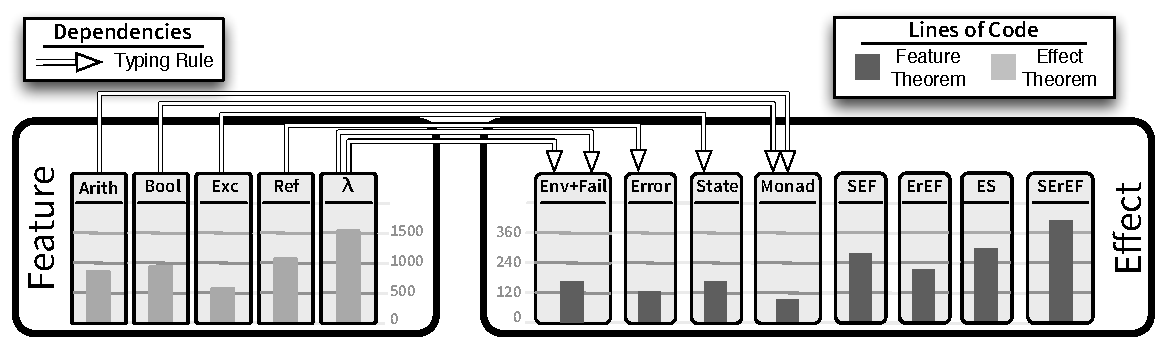
\includegraphics[scale = .85]{src/ModularEffects/CaseStudyFigure.pdf}
   }
  \end{center}
  \caption{Dependency and size information for the features and effects used in the case study.}
  \label{fig:codesize}
\end{figure*}

\section{Case Study}
\label{sec:CaseStudy}

As a demonstration of the \Name~framework, we have built a set of five
reusable language features and combined them to build a family of
languages which includes a mini-ML~\cite{clement86mini-ML} variant
with references and errors. The study includes pure boolean and
arithmetic features as well as effectful features for references,
errors and lambda abstractions.

The study builds twenty eight different combinations of the features which are
all possible combinations with at least one feature providing
values.\footnote{Also available at \url{http://www.cs.utexas.edu/~bendy/3MT}}
Figure~\ref{fig:MiniMLSyntax} presents the syntax of the expressions,
values, and types provided; each line is annotated with the feature
that provides that set of definitions.

Four kinds of feature interactions appear in the case study.

\begin{itemize}

\item The PHOAS representation of binders requires an auxiliary
equivalence relation, the details of which are covered in the MTC
paper~\cite{mtc}. The soundness proofs of language theorems for
languages which include binders proceed by induction over this
equivalence relation instead of expressions. The reusable feature
theorems of other features need to be lifted to this equivalence
relation.

\item The effect theorems that feature an environment
typing $\Sigma$, such as those for state or environment, need a weakening sublemma
which
states
that each well-formed value under
$\Sigma$ is also well-formed under a conservative extension:
\[\Sigma \vdash v ~:~ t  \\ \rightarrow \\
  \Sigma' \supseteq \Sigma \\ \rightarrow \\
  \Sigma' \vdash v ~:~ t \]
\item Inversion lemmas for the well-formed value relation as in the
proof of \ref{thm:FSound} for the boolean feature in
Section \ref{sec:Thm+Reuse} are proven by induction over the
relation.

%% \item The sublemmas of reusable feature theorems for properties such as
%% \textsc{WFM-If-Vc} are
%% proven by induction over the extensible typing relation. When effectful
%% features introduce new judgements to the relation, these new
%% judgements must have proof algebra instances for the sublemmas.

\end{itemize}


The proofs of the first and second kind of feature interactions are
straightforward; the inversion lemmas of the third kind can be
dispatched by tactics hooked into the type class inference algorithm.
%% The last kind of interactions require more work and comprise the
%% biggest part of the code dealing with feature interactions.
%%
%% The presented typing rules for effects satisfy the \textsc{WFM-Bind}
%% property; as previously discussed, it can be used cut down on feature
%% interactions. The lambda feature uses \textsc{WFM-Bind} in its proof
%% of \ref{thm:FSound} instead of targeted sublemmas. The following table
%% shows the number of sublemmas used by the reusable feature theorems,
%% highlighting that the \textsc{WFM-Bind} property provides significantly
%% more convenience despite its stronger assumptions.


The framework itself consists of about 4,400 LoC of which about 2,000
LoC comprise the implementation of the monad transformers and their
algebraic laws. The size in LoC of the implementation of semantic
evaluation and typing functions and the reusable feature theorem for
each language feature is given in the left box in Figure
\ref{fig:codesize}. The right box lists the sizes of the effect
theorems. Each language needs on average 110 LoC to assemble its
semantic functions and soundness proofs from those of its features and
the effect theorem for its set of effects.


\begin{figure}[t]
  \begin{center}
    \begin{minipage}{\columnwidth}
      \begin{center}
        \fbox{
        \hspace{-.3cm}
          \begin{tabular}{r@{~}c@{~}lr}
            {\tt e} & ::= & {\tt $\mathbb{N}$ $|$ e + e} & \textit{Arith}\\
            & $|$ &  {\tt $\mathbb{B}$ $|$ {\bf if} e {\bf then} e {\bf else} e} & \textit{Bool} \\
           %% & $|$ & {\tt {\bf case} e {\bf of \{ z} $\Rightarrow$ e $\mathbf{;}$ {\bf S} n $\Rightarrow$ e\}} & \textit{NatCase}\\
            & $|$ & {\tt {\bf lam} x : T.e $|$ e e $|$ x} & \textit{Lambda}\\
            & $|$ & {\tt {\bf ref} e $|$ !e $|$ e:=e} & \textit{References}\\
            & $|$ & {\tt {\bf try} e {\bf with} e} $|$ {\bf error} & \textit{Errors}\\
           %%  & $|$ & {\tt {\bf fix} x : T.e} & \textit{Recursion}\\
          \end{tabular}
        }
      \end{center}
    \end{minipage}
    \begin{minipage}{\columnwidth}
      \hspace{-.3cm}
    \begin{tabular}{cc}
      \begin{minipage}{.48\columnwidth}
        \fbox{
        \hspace{-.3cm}
          \begin{tabular}{r@{~}c@{~}lr}
            {\tt V} & ::= & {\tt $\mathbb{N}$} & \textit{Arith}\\
            & $|$ &  {\tt $\mathbb{B}$} & \textit{Bool} \\
            & $|$ & {\tt {\bf clos} e $\mathtt{\overline{V}}$} & \textit{Lambda}\\
            & $|$ & {\tt {\bf loc} $\mathbb{N}$} & \textit{References}\\
          \end{tabular}
        }
      \end{minipage} &
      \begin{minipage}{.38\columnwidth}
        \hspace{-.3cm}
        \fbox{
        \hspace{-.3cm}
          \begin{tabular}{r@{~}c@{~}lr}
            {\tt T} & ::= & {\tt \bf Nat} & \textit{Arith}\\
            & $|$ &  {\tt \bf Bool} & \textit{Bool} \\
            & $|$ & {\tt T $\rightarrow$ T} & \textit{Lambda}\\
            & $|$ & {\tt {\bf Ref} T} & \textit{References}\\
          \end{tabular}
        }
      \end{minipage}
    \end{tabular}
    \end{minipage}
  \end{center}
  \caption{mini-ML expressions, values, and types}
  \label{fig:MiniMLSyntax}
\end{figure}


%% \begin{center}
%%   \fbox{
%%   \hspace{-.3cm}
%%     \begin{tabular}{ c c c c c }
%%       \textit{Arith} & \textit{Bool} & \textit{Errors} & \textit{References} & \textit{Lambda} \\
%%       2 & 3 & 0 & 4 & 0 \\
%%     \end{tabular}
%%   }
%% \end{center}
%% Each sublemma of the above table requires on average 50 LoC per effect.

%% ODER: format ==         = "\mathrel{==}"
%% ODER: format /=         = "\neq "
%
%
\makeatletter
\@ifundefined{lhs2tex.lhs2tex.sty.read}%
  {\@namedef{lhs2tex.lhs2tex.sty.read}{}%
   \newcommand\SkipToFmtEnd{}%
   \newcommand\EndFmtInput{}%
   \long\def\SkipToFmtEnd#1\EndFmtInput{}%
  }\SkipToFmtEnd

\newcommand\ReadOnlyOnce[1]{\@ifundefined{#1}{\@namedef{#1}{}}\SkipToFmtEnd}
\usepackage{amstext}
\usepackage{amssymb}
\usepackage{stmaryrd}
\DeclareFontFamily{OT1}{cmtex}{}
\DeclareFontShape{OT1}{cmtex}{m}{n}
  {<5><6><7><8>cmtex8
   <9>cmtex9
   <10><10.95><12><14.4><17.28><20.74><24.88>cmtex10}{}
\DeclareFontShape{OT1}{cmtex}{m}{it}
  {<-> ssub * cmtt/m/it}{}
\newcommand{\texfamily}{\fontfamily{cmtex}\selectfont}
\DeclareFontShape{OT1}{cmtt}{bx}{n}
  {<5><6><7><8>cmtt8
   <9>cmbtt9
   <10><10.95><12><14.4><17.28><20.74><24.88>cmbtt10}{}
\DeclareFontShape{OT1}{cmtex}{bx}{n}
  {<-> ssub * cmtt/bx/n}{}
\newcommand{\tex}[1]{\text{\texfamily#1}}	% NEU

\newcommand{\Sp}{\hskip.33334em\relax}


\newcommand{\Conid}[1]{\mathit{#1}}
\newcommand{\Varid}[1]{\mathit{#1}}
\newcommand{\anonymous}{\kern0.06em \vbox{\hrule\@width.5em}}
\newcommand{\plus}{\mathbin{+\!\!\!+}}
\newcommand{\bind}{\mathbin{>\!\!\!>\mkern-6.7mu=}}
\newcommand{\rbind}{\mathbin{=\mkern-6.7mu<\!\!\!<}}% suggested by Neil Mitchell
\newcommand{\sequ}{\mathbin{>\!\!\!>}}
\renewcommand{\leq}{\leqslant}
\renewcommand{\geq}{\geqslant}
\usepackage{polytable}

%mathindent has to be defined
\@ifundefined{mathindent}%
  {\newdimen\mathindent\mathindent\leftmargini}%
  {}%

\def\resethooks{%
  \global\let\SaveRestoreHook\empty
  \global\let\ColumnHook\empty}
\newcommand*{\savecolumns}[1][default]%
  {\g@addto@macro\SaveRestoreHook{\savecolumns[#1]}}
\newcommand*{\restorecolumns}[1][default]%
  {\g@addto@macro\SaveRestoreHook{\restorecolumns[#1]}}
\newcommand*{\aligncolumn}[2]%
  {\g@addto@macro\ColumnHook{\column{#1}{#2}}}

\resethooks

\newcommand{\onelinecommentchars}{\quad-{}- }
\newcommand{\commentbeginchars}{\enskip\{-}
\newcommand{\commentendchars}{-\}\enskip}

\newcommand{\visiblecomments}{%
  \let\onelinecomment=\onelinecommentchars
  \let\commentbegin=\commentbeginchars
  \let\commentend=\commentendchars}

\newcommand{\invisiblecomments}{%
  \let\onelinecomment=\empty
  \let\commentbegin=\empty
  \let\commentend=\empty}

\visiblecomments

\newlength{\blanklineskip}
\setlength{\blanklineskip}{0.66084ex}

\newcommand{\hsindent}[1]{\quad}% default is fixed indentation
\let\hspre\empty
\let\hspost\empty
\newcommand{\NB}{\textbf{NB}}
\newcommand{\Todo}[1]{$\langle$\textbf{To do:}~#1$\rangle$}

\EndFmtInput
\makeatother
%
%
%
%
%
%
% This package provides two environments suitable to take the place
% of hscode, called "plainhscode" and "arrayhscode". 
%
% The plain environment surrounds each code block by vertical space,
% and it uses \abovedisplayskip and \belowdisplayskip to get spacing
% similar to formulas. Note that if these dimensions are changed,
% the spacing around displayed math formulas changes as well.
% All code is indented using \leftskip.
%
% Changed 19.08.2004 to reflect changes in colorcode. Should work with
% CodeGroup.sty.
%
\ReadOnlyOnce{polycode.fmt}%
\makeatletter

\newcommand{\hsnewpar}[1]%
  {{\parskip=0pt\parindent=0pt\par\vskip #1\noindent}}

% can be used, for instance, to redefine the code size, by setting the
% command to \small or something alike
\newcommand{\hscodestyle}{}

% The command \sethscode can be used to switch the code formatting
% behaviour by mapping the hscode environment in the subst directive
% to a new LaTeX environment.

\newcommand{\sethscode}[1]%
  {\expandafter\let\expandafter\hscode\csname #1\endcsname
   \expandafter\let\expandafter\endhscode\csname end#1\endcsname}

% "compatibility" mode restores the non-polycode.fmt layout.

\newenvironment{compathscode}%
  {\par\noindent
   \advance\leftskip\mathindent
   \hscodestyle
   \let\\=\@normalcr
   \let\hspre\(\let\hspost\)%
   \pboxed}%
  {\endpboxed\)%
   \par\noindent
   \ignorespacesafterend}

\newcommand{\compaths}{\sethscode{compathscode}}

% "plain" mode is the proposed default.
% It should now work with \centering.
% This required some changes. The old version
% is still available for reference as oldplainhscode.

\newenvironment{plainhscode}%
  {\hsnewpar\abovedisplayskip
   \advance\leftskip\mathindent
   \hscodestyle
   \let\hspre\(\let\hspost\)%
   \pboxed}%
  {\endpboxed%
   \hsnewpar\belowdisplayskip
   \ignorespacesafterend}

\newenvironment{oldplainhscode}%
  {\hsnewpar\abovedisplayskip
   \advance\leftskip\mathindent
   \hscodestyle
   \let\\=\@normalcr
   \(\pboxed}%
  {\endpboxed\)%
   \hsnewpar\belowdisplayskip
   \ignorespacesafterend}

% Here, we make plainhscode the default environment.

\newcommand{\plainhs}{\sethscode{plainhscode}}
\newcommand{\oldplainhs}{\sethscode{oldplainhscode}}
\plainhs

% The arrayhscode is like plain, but makes use of polytable's
% parray environment which disallows page breaks in code blocks.

\newenvironment{arrayhscode}%
  {\hsnewpar\abovedisplayskip
   \advance\leftskip\mathindent
   \hscodestyle
   \let\\=\@normalcr
   \(\parray}%
  {\endparray\)%
   \hsnewpar\belowdisplayskip
   \ignorespacesafterend}

\newcommand{\arrayhs}{\sethscode{arrayhscode}}

% The mathhscode environment also makes use of polytable's parray 
% environment. It is supposed to be used only inside math mode 
% (I used it to typeset the type rules in my thesis).

\newenvironment{mathhscode}%
  {\parray}{\endparray}

\newcommand{\mathhs}{\sethscode{mathhscode}}

% texths is similar to mathhs, but works in text mode.

\newenvironment{texthscode}%
  {\(\parray}{\endparray\)}

\newcommand{\texths}{\sethscode{texthscode}}

% The framed environment places code in a framed box.

\def\codeframewidth{\arrayrulewidth}
\RequirePackage{calc}

\newenvironment{framedhscode}%
  {\parskip=\abovedisplayskip\par\noindent
   \hscodestyle
   \arrayrulewidth=\codeframewidth
   \tabular{@{}|p{\linewidth-2\arraycolsep-2\arrayrulewidth-2pt}|@{}}%
   \hline\framedhslinecorrect\\{-1.5ex}%
   \let\endoflinesave=\\
   \let\\=\@normalcr
   \(\pboxed}%
  {\endpboxed\)%
   \framedhslinecorrect\endoflinesave{.5ex}\hline
   \endtabular
   \parskip=\belowdisplayskip\par\noindent
   \ignorespacesafterend}

\newcommand{\framedhslinecorrect}[2]%
  {#1[#2]}

\newcommand{\framedhs}{\sethscode{framedhscode}}

% The inlinehscode environment is an experimental environment
% that can be used to typeset displayed code inline.

\newenvironment{inlinehscode}%
  {\(\def\column##1##2{}%
   \let\>\undefined\let\<\undefined\let\\\undefined
   \newcommand\>[1][]{}\newcommand\<[1][]{}\newcommand\\[1][]{}%
   \def\fromto##1##2##3{##3}%
   \def\nextline{}}{\) }%

\newcommand{\inlinehs}{\sethscode{inlinehscode}}

% The joincode environment is a separate environment that
% can be used to surround and thereby connect multiple code
% blocks.

\newenvironment{joincode}%
  {\let\orighscode=\hscode
   \let\origendhscode=\endhscode
   \def\endhscode{\def\hscode{\endgroup\def\@currenvir{hscode}\\}\begingroup}
   %\let\SaveRestoreHook=\empty
   %\let\ColumnHook=\empty
   %\let\resethooks=\empty
   \orighscode\def\hscode{\endgroup\def\@currenvir{hscode}}}%
  {\origendhscode
   \global\let\hscode=\orighscode
   \global\let\endhscode=\origendhscode}%

\makeatother
\EndFmtInput
%
%
%
% First, let's redefine the forall, and the dot.
%
%
% This is made in such a way that after a forall, the next
% dot will be printed as a period, otherwise the formatting
% of `comp_` is used. By redefining `comp_`, as suitable
% composition operator can be chosen. Similarly, period_
% is used for the period.
%
\ReadOnlyOnce{forall.fmt}%
\makeatletter

% The HaskellResetHook is a list to which things can
% be added that reset the Haskell state to the beginning.
% This is to recover from states where the hacked intelligence
% is not sufficient.

\let\HaskellResetHook\empty
\newcommand*{\AtHaskellReset}[1]{%
  \g@addto@macro\HaskellResetHook{#1}}
\newcommand*{\HaskellReset}{\HaskellResetHook}

\global\let\hsforallread\empty

\newcommand\hsforall{\global\let\hsdot=\hsperiodonce}
\newcommand*\hsperiodonce[2]{#2\global\let\hsdot=\hscompose}
\newcommand*\hscompose[2]{#1}

\AtHaskellReset{\global\let\hsdot=\hscompose}

% In the beginning, we should reset Haskell once.
\HaskellReset

\makeatother
\EndFmtInput

% format runC         = "run\mathbb{C}_{\scalebox{0.6}{T}}"
% format C            = "\mathbb{C}_{\scalebox{0.6}{T}}"
%%format R            = "\mathbb{R}_{\scalebox{0.6}{T}}"


\section{Related and Future Work}

\paragraph{DGP in proof-assistants}

Datatype-generic programming started out as a form of language
extension such as PolyP \cite{jansson:polyp} or Generic Haskell
\cite{loh:dsgh}. Yet Haskell has turned out to be powerful enough to
implement datatype-generic programming in the language itself and over
the time a vast number of DGP libraries for Haskell have been proposed
\cite{cheney:ligd,syb,emgm,multirec,instantgenerics,uniplate,genericderiving}. Compared
with a language extension, a library is much easier to develop and
maintain.

Using the flexibility of dependent-types there are multiple proposals
for performing datatype-generic programming in proof assistants
\cite{dgpcoq,altenkirch:gpwdtp,benke:universes,loh:gpif,indexedcontainers}. This
setting not only allows the implementation of generic functions, but
also of generic proofs. The approaches vary in terms of how strictly
they follow the positivity or termination restrictions imposed by the
proof assistant. Some circumvent the type-checker at various points to
simplify the development or presentation while others put more effort
in convincing the type-checker and termination checker of the validity
\cite{ertt}. However, in all of the proposals there does not seem to
be any fundamental problem caused by the restrictions.


\paragraph{DGP for modular proofs}

Modularly composing semantics and proofs about the semantics has also
been addressed by \cite{schwaab:mtp} in the context of programming
language meta-theory. They perform their development in Agda and
similar to our approach they also use a universe approach based on
polynomial functors to represent modular datatypes. They split
relations for small-step operational semantics and well-typing on a
feature basis. However, the final fixed points are constructed manually
instead of having a generic representation of inductive families.

Using Coq's type classes both MTC and our approach also allow for more
automation in the final composition of datatypes, functions and
proofs. Agda features instance arguments that can be used to replace
type classes in various cases. However, the current implementation
does not perform recursive resolution and as a result Agda does not
support automation of the composition to the extent that is needed for
DTC-like approaches.


\paragraph{Combining different DGP approaches}

We have shown an embedding of the universe of polynomial functors into
the universe of containers. Similar inclusions between universes have
been done in the literature \cite{morris:cspf}. Magalh\~aes and L\"oh
\cite{jpm:fcadgp} have ported several popular DGP approaches from
Haskell to Agda and performed a formal comparison by proving inclusion
relations between the approaches.

DGP approaches differ in terms of the class of datatypes they capture and the
set of generic functions that can be implemented for them. Generic functions
can be transported from a universe into a sub-universe. However, we are not
aware of any DGP library with a systematic treatment of universes where each generic
function is defined on the most general universe that supports that function.


\paragraph{DGP for abstract syntax}

We have shown how to obtain more reuse by complementing modular
definitions with a generic equality function and generic proofs of its
properties. Of course more generic functionality like traversals,
pretty-printing, parsing etc. can be covered by means of
datatype-generic programming.

One very interesting idea is to use datatype-generic programming to
handle variable binding \cite{cheney:synp,unbound}. Variable
binding is an ubiquitous aspect of programming languages. Moreover, a
lot of functionality like variable substitutions and free variable
calculations is defined for many languages. Licata and Harper
\cite{licata:ubc} and Keuchel and Jeuring \cite{sk:gcasr} define
universes for datatypes with binding in Agda. Lee et al.~\cite{gmeta}
develop a framework for first-order representations of variable
binding in Coq that is based on the universe of regular tree types
\cite{ertt} and that provides many of the so-called
\emph{infrastructure lemmas} required when mechanizing programming
language meta-theory.

An interesting direction for future work is to extend these approaches
to capture variable binding in the indices of relations on abstract
syntax and use this as the underlying representation of extensible
datatypes and extensible logical relations and thereby complementing
modular functions with generic proofs about variable binding.


\paragraph{Automatic derivation of instances}

Most, if not all, generic programming libraries in Haskell use Template
Haskell to derive the generic representation of user-defined types and
to derive the conversion functions between them.

The GMeta \cite{gmeta} framework includes a standalone tool that also
performs this derivation for Coq. Similarly we also like to be able
to derive instances for the \ensuremath{\Conid{Container}} and \ensuremath{\Conid{Polynomial}} classes
automatically.


Formally mechanizing proofs can be very tedious and the amount of work
required for larger developments is excruciating. Meta-Theory \`a la Carte
is a framework for modular reusable components for use in
mechanizations. It builds on the Datatypes \`a la Carte approach to solve
an extended version of the expression problem. MTC allows modular
definitions of datatypes, semantic functions and logical relations and
furthermore modular inductive proofs.

MTC uses extensible Church-encodings to overcome conservative restrictions
imposed by the Coq proof-assistant. This approach has shortcomings
in terms of confidence in the definitions and in terms of usability. This
paper addresses these shortcomings by using datatype-generic
programming techniques to replace Church-encodings as the underlying representation
of type-level fixed points. Our approach avoids impredicativity, adequately
encodes fixed points and leads to stronger induction principles by
exploiting DGP approaches that capture only strictly-positive functors.

Working with generic structure representation has the added benefit that
we can implement generic functions like equality and generic proofs once and for all.



%%% Local Variables:
%%% mode: latex
%%% TeX-master: "../main"
%%% End:
